%versi 2 (8-10-2016)
\setcounter{secnumdepth}{3}

\chapter{Landasan Teori}
\label{chap:teori}

%2.1 WCAG 2.1%
\section{\textit{WCAG 2.1} \cite{WCAG:2.1}}
\label{sec:wcag_2.1}  
\textit{WCAG} 2.1 dibuat untuk meningkatkan versi sebelumnya yaitu \textit{WCAG} 2.0. Pada \textit{WCAG} 2.1 terdapat penambahan kriteria sukses baru beserta definisi-definisi pendukungnya, pedoman untuk mengatur penambahan, dan beberapa tambahan pada bagian tingkat kepatuhan. Dalam \textit{WCAG} 2.1 terdapat 3 tingkat kriteria sukses yaitu A, AA, dan AAA yang digunakan sebagai acuan untuk menilai tingkat kepatuhan sebuah situs web terhadap \textit{WCAG} 2.1. Agar suatu halaman web dikatakan mematuhi \textit{WCAG} 2.1, semua persyaratan kepatuhan berikut haruslah dipenuhi:
\begin{itemize}
	\item Tingkat Kepatuhan; salah satu dari tingkat kepatuhan berikut dipenuhi seutuhnya:
	\begin{itemize}
		\item Tingkat A: Untuk tingkat A (tingkat paling rendah), diperoleh jika halaman web berhasil mematuhi seluruh kriteria sukses tingkat A atau tersedia versi alternatif yang sesuai.
		\item Tingkat AA: Untuk tingkat AA, diperoleh jika halaman web berhasil mematuhi seluruh kriteria sukses tingkat A dan AA atau tersedia versi alternatif tingkat AA yang sesuai.
		\item Tingkat AAA: Untuk tingkat AAA, diperoleh jika halaman web berhasil mematuhi seluruh kriteria sukses tingkat A, AA, dan AAA atau tersedia versi alternatif tingkat AAA yang sesuai.
	\end{itemize}
	Sebagai catatan: tingkat kepatuhan AAA amat tidak dianjurkan untuk diterapkan sebagai kebijakan umum untuk keseluruhan situs web, karena amat tidak mungkin memenuhi semua kriteria sukses tingkat AAA untuk beberapa jenis konten.
	\item Halaman Lengkap: tingkat kepatuhan berlaku untuk seluruh halaman web dan tidak boleh ada halaman yang dikecualikan.
	\item Proses Lengkap: untuk halaman web yang merupakan satu dari beberapa halaman yang merupakan proses, semua halaman web dalam proses tersebut harus mematuhi tingkat yang ditentukan atau lebih baik. Contohnya adalah halaman pembayaran pada sebuah website jual beli, seluruh halaman yang merupakan proses dari proses berbelanja tersebut harus mematuhi tingkat kepatuhan yang ditentukan.
	\item \textit{Web Content Technologies}\footnote{Mekanisme untuk \textit{user agent} menyajikan atau menjalankan instruksi yang berupa kode. Meliputi bahasa \textit{markup}, format data, atau bahasa pemrograman. Contohnya \textit{HTML, CSS, SVG, PNG, PDF, Flash, dan JavaScript}} mendukung aksesibilitas: Hanya cara-cara pemanfaatan \textit{Web Content Technologies} yang mendukung aksesibilitas yang dapat diandalkan untuk memenuhi kriteria sukses. Informasi dan fungsionalitas yang tersedia dalam cara yang tidak mendukung aksesibilitas, juga harus tersedia dalam cara yang mendukung aksesibilitas.
	\item Tidak Menghambat: jika \textit{Web Content Technologies} yang dimanfaatkan tidak mendukung aksesibilitas, maka pemanfaatan tersebut tidak boleh menghalangi kemampuan pengguna untuk mengakses sisa halaman. Sebagai tambahan, halaman web tersebut secara keseluruhan harus tetap memenuhi persyaratan kepatuhan dalam kondisi-kondisi sebagai berikut:
	\begin{enumerate}
		\item \textit{Web Content Technologies} yang tidak diandalkan untuk mematuhi persyaratan kepatuhan, dinyalakan oleh \textit{user agent}\footnote{Perangkat lunak yang mengambil konten web dan menyajikannya kepada pengguna, contohnya \textit{web browsers, media player, plug-ins}, dan program lainnya termasuk juga teknologi alat bantu}.
		\item \textit{Web Content Technologies} yang tidak diandalkan untuk mematuhi persyaratan kepatuhan, dimatikan oleh \textit{user agent}.
		\item \textit{Web Content Technologies} yang tidak diandalkan untuk mematuhi persyaratan kepatuhan, tidak didukung oleh \textit{user agent}.
	\end{enumerate}
\end{itemize}

Dalam \textit{WCAG} 2.1 terdapat tujuh puluh delapan poin kriteria sukses yang kemudian dikelompokkan dalam empat kategori besar yaitu \textit{perceivable}, \textit{operable}, \textit{understandable}, dan \textit{robust}. Dalam masing-masing kategori, setiap kriteria sukses dikelompokkan lagi ke dalam kategori-kategori kecil yang lebih spesifik. Pembagian dan pengelompokan ini dibuat agar dapat memenuhi berbagai kebutuhan dari khalayak banyak yang sangat beragam yang menggunakan \textit{WCAG} seperti pengembang dan desainer web, pembuat kebijakan, agen pembeli, tenaga pendidik, dan pelajar maupun mahasiswa. Pada subbab-subbab berikutnya membahas satu per satu poin kriteria sukses berdasarkan kategorinya.

%2.1.1 Perceivable%
\subsection{\textit{Perceivable}}
\label{sec:perceivable}
Pada subbab ini dibahas kriteria-kriteria sukses yang termasuk ke dalam kategori \textit{perceivable}. Kategori ini mensyaratkan agar informasi dan komponen antarmuka pengguna disajikan dengan cara yang bisa dipahami oleh pengguna. Terdapat dua puluh sembilan poin kriteria sukses yang dikelompokkan ke dalam empat kategori kecil yaitu \textit{text alternatives}, \textit{time-based media}, \textit{adaptable}, dan \textit{distinguishable}.

%2.1.1.1 Text Alternatives%
\subsubsection{\textit{Text Alternatives}}
\label{sec:text_alternatives}
Pada subbab ini dibahas kriteria sukses yang termasuk ke dalam kategori \textit{text alternatives}. Kategori ini mensyaratkan agar tersedia teks alternatif untuk setiap konten yang bukan merupakan teks. Terdapat satu poin kriteria sukses di dalam kategori ini.

\paragraph{Kriteria Sukses 1.1.1 \textit{Non-text Content}}
\label{sec:kriteria_sukses_1.1.1}
(Level A)\\

Semua konten yang bukan merupakan teks yang disajikan ke pengguna harus mempunyai teks alternatif. Teks alternatif tersebut harus dapat menyajikan informasi dengan tujuan yang sama, kecuali untuk situasi-situasi berikut:
\begin{itemize}
	\item Jika konten merupakan sebuah kontrol atau menerima \textit{input} dari pengguna, maka konten tersebut harus mempunyai nama yang menjelaskan tujuannya yang dapat diidentifikasi oleh teknologi alat bantu.
	\item Jika konten merupakan media berbasis waktu\footnote{Media yang berkaitan dengan waktu, contohnya rekaman audio dan rekaman video}, maka setidaknya teks alternatif menyediakan identifikasi deskriptif dari konten tersebut.
	\item Jika konten merupakan tes atau latihan, yang akan mengungkap jawabannya jika disajikan dalam bentuk teks, maka setidaknya teks alternatif menyajikan identifikasi deskriptif dari konten tersebut. Contohnya sebuah latihan menebak gambar yang mengharuskan pengguna untuk memberikan jawaban berdasarkan gambar yang dilihatnya. Dalam hal ini teks alternatif pada gambar tersebut tidak boleh memberikan jawabannya, melainkan memberikan petunjuk mengenai tujuan dari adanya gambar tersebut.
	\item Jika tujuan utama konten untuk menciptakan pengalaman sensorik tertentu, maka setidaknya teks alternatif menyediakan identifikasi deskriptif untuk konten tersebut. Contohnya adalah sebuah lukisan.
	\item Jika konten adalah \textit{CAPTCHA (Completely Automatic Public Turing Test to Tell Computers and Humans Apart)} yang bertujuan untuk mengonfirmasi bahwa konten sedang diakses oleh manusia dan bukan oleh komputer, maka tersedia teks alternatif yang menjelaskan tujuan dari konten tersebut, serta tersedia \textit{CAPTCHA} dalam bentuk lain yang memberikan \textit{output} untuk berbagai jenis indera agar dapat mengakomodasi berbagai disabilitas.
	\item Jika konten hanya merupakan dekorasi yang digunakan untuk format visual atau tidak disajikan kepada pengguna, maka konten tersebut diimplementasikan dengan cara yang dapat diabaikan oleh teknologi alat bantu.
\end{itemize}
%End of 2.1.1.1 Text Alternatives%

%2.1.1.2 Time-based Media%
\subsubsection{\textit{Time-based Media}}
\label{sec:time_based_media}
Pada subbab ini dibahas kriteria sukses yang termasuk ke dalam kategori \textit{time-based media}. Kategori ini mensyaratkan agar tersedia alternatif untuk media berbasis waktu. Terdapat sembilan poin kriteria sukses di dalam kategori ini.

\paragraph{Kriteria Sukses 1.2.1 \textit{Audio-only and Video-only (Prerecorded)}}
\label{sec:kriteria_sukses_1.2.1}
(Level A)\\

Untuk media rekaman berupa audio saja dan video saja yang bukan merupakan media alternatif untuk teks, maka terdapat beberapa ketentuan yang berlaku: 
\begin{itemize}
	\item Media rekaman audio saja: Tersedia alternatif yang isinya mewakili informasi yang sama dengan konten yang disajikan.
	\item Media rekaman video saja: Tersedia alternatif atau audio yang isinya mewakili informasi yang sama dengan konten yang disajikan.
\end{itemize}

\paragraph{Kriteria Sukses 1.2.2 \textit{Captions (Prerecorded)}}
\label{sec:kriteria_sukses_1.2.2}
(Level A)\\

Tersedia \textit{captions} untuk semua konten rekaman audio, kecuali bila media tersebut merupakan media alternatif untuk teks dan dilabeli dengan jelas.

\paragraph{Kriteria Sukses 1.2.3 \textit{Audio Description or Media Alternative (Prerecorded)}}
\label{sec:kriteria_sukses_1.2.3}
(Level A)\\

Tersedia alternatif untuk konten yang merupakan media berbasis waktu atau jika konten merupakan rekaman video maka tersedia deskriptif audio untuk konten tersebut, kecuali jika media tersebut merupakan media alternatif untuk teks dan dilabeli dengan jelas.

\paragraph{Kriteria Sukses 1.2.4 \textit{Captions (Live)}}
\label{sec:kriteria_sukses_1.2.4}
(Level AA)\\

Tersedia \textit{captions} untuk semua konten audio yang merupakan siaran langsung.

\paragraph{Kriteria Sukses 1.2.5 \textit{Audio Description (Prerecorded)}}
\label{sec:kriteria_sukses_1.2.5}
(Level AA)\\

Tersedia deskriptif audio untuk semua konten rekaman video.

\paragraph{Kriteria Sukses 1.2.6 \textit{Sign Language (Prerecorded)}}
\label{sec:kriteria_sukses_1.2.6}
(Level AAA)\\

Tersedia penafsiran bahasa isyarat untuk semua konten rekaman audio. 

\paragraph{Kriteria Sukses 1.2.7 \textit{Extended Audio Description (Prerecorded)}}
\label{sec:kriteria_sukses_1.2.7}
(Level AAA)\\

Tersedia tambahan deskriptif audio untuk semua konten rekaman video ketika jeda suara latar depan yang ada tidak cukup untuk menyampaikan maksud video karena terdapat banyak peristiwa dengan tempo yang cepat dalam video tersebut. Tambahan deskriptif audio ini disediakan dengan cara menghentikan sementara video yang sedang berjalan.

\paragraph{Kriteria Sukses 1.2.8 \textit{Media Alternative (Prerecorded)}}
\label{sec:kriteria_sukses_1.2.8}
(Level AAA)\\

Tersedia alternatif untuk semua media rekaman dan media rekaman video saja.

\paragraph{Kriteria Sukses 1.2.9 \textit{Audio-only (Live)}}
\label{sec:kriteria_sukses_1.2.9}
(Level AAA)\\

Tersedia alternatif yang menyajikan informasi yang sama dengan konten audio saja yang merupakan siaran langsung.
%End of 2.1.1.2 Time-based Media%

%2.1.1.3 Adaptable%
\subsubsection{\textit{Adaptable}}
\label{sec:adaptable}
Pada subbab ini dibahas kriteria sukses yang termasuk ke dalam kategori \textit{adaptable}. Kategori ini mensyaratkan agar konten dapat disajikan dalam berbagai cara (misalnya tata letak yang lebih sederhana) tanpa kehilangan informasi atau struktur konten tersebut. Terdapat enam poin kriteria sukses di dalam kategori ini.

\paragraph{Kriteria Sukses 1.3.1 \textit{Info and Relationships}}
\label{sec:kriteria_sukses_1.3.1}
(Level A)\\

Informasi, struktur halaman web, dan hubungan antar konten yang disajikan kepada pengguna harus dapat tetap terjaga meskipun format penyampaiannya kepada pengguna berbeda-beda.

\paragraph{Kriteria Sukses 1.3.2 \textit{Meaningful Sequence}}
\label{sec:kriteria_sukses_1.3.2}
(Level A)\\

Jika urutan konten yang disajikan memengaruhi makna konten tersebut, maka urutan membaca yang benar harus dapat diidentifikasi oleh teknologi alat bantu.

\paragraph{Kriteria Sukses 1.3.3 \textit{Sensory Characteristics}}
\label{sec:kriteria_sukses_1.3.3}
(Level A)\\

Instruksi yang tersedia untuk memahami maupun mengoperasikan konten tidak hanya mengandalkan satu karakteristik indera seperti bentuk, ukuran, lokasi visual, orientasi, atau suara.

\paragraph{Kriteria Sukses 1.3.4 \textit{Orientation}}
\label{sec:kriteria_sukses_1.3.4}
(Level AA)\\

Konten tidak membatasi tampilan dan pengoperasiannya hanya untuk satu orientasi tampilan saja, seperti \textit{portrait} atau \textit{landscape}, kecuali jika orientasi tampilan tertentu bersifat esensial.

\paragraph{Kriteria Sukses 1.3.5 \textit{Identify Input Purpose}}
\label{sec:kriteria_sukses_1.3.5}
(Level AA)\\

Tujuan dari setiap kolom \textit{input} yang mengumpulkan informasi tentang pengguna dapat ditentukan secara terprogram\footnote{Ditentukan oleh perangkat lunak berdasarkan data dari pembuat konten yang disediakan sedemikian rupa sehingga dapat diidentifikasi oleh beragam \textit{user agent} termasuk teknologi alat bantu yang kemudian disajikan kepada pengguna dengan berbagai macam mode}.

\paragraph{Kriteria Sukses 1.3.6 \textit{Identify Purpose}}
\label{sec:kriteria_sukses_1.3.6}
(Level AAA)\\

Pada konten yang diimplementasikan dengan menggunakan bahasa \textit{markup}, tujuan dari komponen antarmuka pengguna, ikon, dan bagian-bagian konten dapat ditentukan secara terprogram.
%End of 2.1.1.3 Adaptable%

%2.1.1.4 Distinguishable%
\subsubsection{\textit{Distinguishable}}
\label{sec:distinguishable}
Pada subbab ini dibahas kriteria sukses yang termasuk ke dalam kategori \textit{distinguishable}. Kategori ini mensyaratkan agar konten yang disajikan kepada pengguna dapat dilihat dan didengar dengan mudah oleh pengguna, termasuk juga kemudahan dalam memisahkan latar depan dari latar belakang. Terdapat tiga belas poin kriteria sukses di dalam kategori ini.

\paragraph{Kriteria Sukses 1.4.1 \textit{Use of Color}}
\label{sec:kriteria_sukses_1.4.1}
(Level A)\\

Warna tidak digunakan sebagai satu-satunya cara yang digunakan untuk menyampaikan informasi secara visual, menandai suatu tindakan, meminta respons, atau membedakan elemen visual.

\paragraph{Kriteria Sukses 1.4.2 \textit{Audio Control}}
\label{sec:kriteria_sukses_1.4.2}
(Level A)\\

Jika pada halaman web terdapat audio yang diputar otomatis selama lebih dari 3 detik, maka harus tersedia mekanisme untuk memberi jeda atau memberhentikan audio tersebut, atau tersedia mekanisme untuk mengatur volume audio tersebut.

\paragraph{Kriteria Sukses 1.4.3 \textit{Contrast (Minimum)}}
\label{sec:kriteria_sukses_1.4.3}
(Level AA)\\

Penyajian visual dari teks dan gambar teks\footnote{Teks yang telah diubah ke dalam bentuk bukan teks yaitu gambar dengan tujuan untuk mendapatkan efek visual tertentu} memiliki rasio kontras setidaknya 4.5:1, kecuali untuk ketentuan berikut:

\begin{itemize}
	\item Teks yang berukuran besar dan gambar teks yang berukuran besar harus memiliki rasio kontras setidaknya 3:1.
	\item Teks atau gambar teks yang hanya merupakan dekorasi atau bagian gambar yang mengandung konten visual lain yang penting, tidak wajib memenuhi persyaratan kontras apa pun.
	\item Teks yang merupakan bagian dari logo atau nama merek tidak wajib memenuhi persyaratan kontras apa pun.
\end{itemize}

Nilai rasio kontras dapat berkisar antara 1 hingga 21 dan biasa dituliskan sebagai 1:1 hingga 21:1. Rasio kontras antara warna latar depan dan warna latar belakang dapat dihitung dengan menggunakan rumus berikut:
\[
	Rasio\ kontras = (L1 + 0.05) \div (L2 + 0.05)	
\]

Di mana L1 adalah \textit{relative luminance} dari warna yang lebih terang dan L2 adalah \textit{relative luminance} dari warna yang lebih gelap.

\textit{Relative luminance} adalah kecerahan relatif di titik mana pun pada ruang warna, dengan nol untuk warna hitam yang paling gelap dan satu untuk warna putih yang paling terang. Untuk ruang warna sRGB, \textit{relative luminance} suatu warna dihitung dengan rumus berikut:
\[
	L = 0.2126 \times R + 0.7152 \times G + 0.0722 \times B
\]

Dengan R, G, dan B didefinisikan sebagai berikut:
\[
	R=\left\{
	\begin{array}{rr}
	R_{sRGB}\div 12.92,\ \ R_{sRGB}\le 0.03928 \\ 
	{{((R}_{sRGB}\ +0.055)\div 1.055)}^{2.4},\ \ R_{sRGB}>0.03928
	\end{array}
	\right.
\]
\[
	G=\left\{
	\begin{array}{rr}
	G_{sRGB}\div 12.92,\ \ G_{sRGB}\le 0.03928 \\ 
	{{((G}_{sRGB}\ +0.055)\div 1.055)}^{2.4},\ \ G_{sRGB}>0.03928
	\end{array}
	\right.
\]
\[
	B=\left\{
	\begin{array}{rr}
	B_{sRGB}\div 12.92,\ \ B_{sRGB}\le 0.03928 \\ 
	{{((B}_{sRGB}\ +0.055)\div 1.055)}^{2.4},\ \ B_{sRGB}>0.03928
	\end{array}
	\right.
\]

dan RsRGB, GsRGB, dan BsRGB didefinisikan sebagai:
\[
	R_{sRGB} = R_{8bit}\div 255
\]
\[
	G_{sRGB} = G_{8bit}\div 255
\]
\[
	B_{sRGB} = B_{8bit}\div 255
\] 

\paragraph{Kriteria Sukses 1.4.4 \textit{Resize text}}
\label{sec:kriteria_sukses_1.4.4}
(Level AA)\\

Selain \textit{captions} dan gambar teks, teks harus dapat diubah ukurannya tanpa teknologi alat bantu hingga 200 persen, tanpa kehilangan fungsionalitas ataupun sebagian kontennya.

\paragraph{Kriteria Sukses 1.4.5 \textit{Images of Text}}
\label{sec:kriteria_sukses_1.4.5}
(Level AA)\\

Jika teknologi yang digunakan dapat menyajikan konten visual, maka yang digunakan untuk menyampaikan informasi adalah teks, bukan gambar teks, kecuali untuk ketentuan berikut:

\begin{itemize}
	\item Gambar teks dapat disesuaikan secara visual sesuai kebutuhan pengguna;
	\item Wujud tertentu dari teks bersifat esensial terhadap informasi yang disampaikan.
\end{itemize}

\paragraph{Kriteria Sukses 1.4.6 \textit{Contrast (Enhanced)}}
\label{sec:kriteria_sukses_1.4.6}
(Level AAA)\\

Penyajian visual dari teks dan gambar teks memiliki rasio kontras setidaknya 7:1, kecuali untuk ketentuan berikut:

\begin{itemize}
	\item Teks yang berukuran besar dan gambar teks yang berukuran besar harus memiliki rasio kontras setidaknya 4.5:1.
	\item Teks atau gambar teks yang hanya merupakan dekorasi atau bagian gambar yang mengandung konten visual lain yang penting, tidak wajib memenuhi persyaratan kontras apa pun.
	\item Teks yang merupakan bagian dari logo atau nama merek tidak wajib memenuhi persyaratan kontras apa pun.
\end{itemize}

Perhitungan rasio kontras antara warna latar depan dan warna latar belakang beserta contohnya dapat dilihat pada subbab \ref{sec:kriteria_sukses_1.4.3}.

\paragraph{Kriteria Sukses 1.4.7 \textit{Low or No Background Audio}}
\label{sec:kriteria_sukses_1.4.7}
(Level AAA)\\

Untuk konten rekaman audio yang mengandung ucapan di latar depan, bukan merupakan audio untuk \textit{CAPTCHA} atau audio untuk logo, dan bukan merupakan vokalisasi untuk ekspresi musikal seperti nyanyian atau rap, maka harus memiliki setidaknya salah satu dari ketentuan berikut:

\begin{itemize}
	\item Audio tidak mengandung suara latar belakang.
	\item Jika terdapat suara latar belakang maka suara tersebut dapat dimatikan.
	\item Jika terdapat suara latar belakang maka suara latar belakang tersebut harus setidaknya 20 desibel lebih rendah dari konten ucapan di latar depan, kecuali untuk suara-suara yang muncul sesekali dan hanya berdurasi satu atau dua detik.
\end{itemize}

\paragraph{Kriteria Sukses 1.4.8 \textit{Visual Presentation}}
\label{sec:kriteria_sukses_1.4.8}
(Level AAA)\\

Untuk tampilan sebuah kumpulan teks, harus tersedia mekanisme untuk mencapai tujuan-tujuan berikut:

\begin{itemize}
	\item Warna latar depan dan belakang dapat dipilih oleh pengguna.
	\item Lebarnya tidak lebih dari 80 karakter atau \textit{glyphs} (40 jika karakter \textit{CJK}\footnote{Chinese, Japanese, Korean}).
	\item Teks tidak rata kiri-kanan.
	\item Awal paragraf menjorok masuk minimal satu setengah spasi, jarak setiap paragraf minimal satu setengah kali jarak setiap baris.
	\item Teks dapat diperbesar hingga 200 persen tanpa teknologi alat bantu, namun tetap memungkinkan pengguna untuk membaca baris teks tersebut tanpa perlu melakukan \textit{scroll} halaman secara horizontal.
\end{itemize}

\paragraph{Kriteria Sukses 1.4.9 \textit{Images of Text (No Exception)}}
\label{sec:kriteria_sukses_1.4.9}
(Level AAA)\\

Gambar teks hanya digunakan untuk dekorasi semata atau ketika wujud tertentu dari teks bersifat esensial dalam menyampaikan informasi.

\paragraph{Kriteria Sukses 1.4.10 \textit{Reflow}}
\label{sec:kriteria_sukses_1.4.10}
(Level AA)\\

Konten dapat disajikan tanpa kehilangan fungsionalitas ataupun sebagian konten, dan tanpa memerlukan \textit{scrolling} dalam dua dimensi untuk:

\begin{itemize}
	\item Konten \textit{scrolling} vertikal dengan lebar setara 320 piksel \textit{CSS};
	\item Konten \textit{scrolling} horizontal dengan tinggi setara 256 piksel \textit{CSS}.
\end{itemize}

Kecuali untuk bagian-bagian konten yang memerlukan tata letak dua dimensi untuk menjelaskan makna atau penggunaannya.

\paragraph{Kriteria Sukses 1.4.11 \textit{Non-text Contrast}}
\label{sec:kriteria_sukses_1.4.11}
(Level AA)\\

Penyajian visual pada komponen antarmuka pengguna dan objek grafis harus memiliki rasio kontras setidaknya 3:1 terhadap warna yang berdekatan, kecuali jika:

\begin{itemize}
	\item Komponen antarmuka pengguna tidak aktif atau ketika penampilan komponen tersebut ditentukan oleh \textit{user agent} dan tidak dimodifikasi oleh pembuat konten.
	\item Pada objek grafis, penyajian tertentu bersifat esensial untuk informasi yang disampaikan.
\end{itemize}

Perhitungan rasio kontras antara warna latar depan dan warna latar belakang beserta contohnya dapat dilihat pada subbab \ref{sec:kriteria_sukses_1.4.3}.

\paragraph{Kriteria Sukses 1.4.12 \textit{Text Spacing}}
\label{sec:kriteria_sukses_1.4.12}
(Level AA)\\

Pada konten yang diimplementasikan dengan menggunakan bahasa \textit{markup} yang mendukung properti \textit{style} di bawah ini, saat dilakukan pengaturan untuk properti-properti ini tidak boleh ada fungsionalitas ataupun konten yang hilang:

\begin{itemize}
	\item Tinggi baris (jarak antara baris) setidaknya 1.5 kali ukuran tulisan;
	\item Jarak antara paragraf setidaknya 2 kali ukuran tulisan;
	\item Jarak antara huruf setidaknya 0.12 kali ukuran tulisan;
	\item Jarak antara kata setidaknya 0.16 kali ukuran tulisan.
\end{itemize}

Pengecualian: Teks yang tidak menggunakan satu atau lebih properti \textit{style} ini, dapat disesuaikan dengan menggunakan properti yang tersedia untuk teks tersebut.

\paragraph{Kriteria Sukses 1.4.13 \textit{Content on Hover or Focus}}
\label{sec:kriteria_sukses_1.4.13}
(Level AA)\\

Ketika elemen pada halaman web mendapat fokus dari kursor atau fokus \textit{keyboard} dan kemudian muncul konten tambahan (contohnya \textit{tooltip}), ketentuan berikut ini harus terpenuhi:

\begin{itemize}
	\item Tersedia mekanisme untuk menyingkirkan konten tambahan tersebut tanpa perlu memindahkan kursor atau fokus \textit{keyboard}, kecuali jika konten tambahan itu menginformasikan kesalahan \textit{input} atau tidak menghalangi maupun mengganti konten lain;
	\item Jika kursor dapat memicu konten tambahan, maka kursor dapat dipindahkan ke konten tambahan tanpa membuat konten tambahan tersebut menghilang;
	\item Konten tambahan tetap tampak sampai penunjuk atau pemicu fokus dihapus, disingkirkan pengguna, atau informasinya sudah tidak valid.
\end{itemize}

Pengecualian: Penyajian visual pada konten tambahan diatur oleh \textit{user agent} dan tidak dimodifikasi oleh pembuat konten.

%End of 2.1.1.4 Distinguishable%

%End of 2.1.1 Perceivable%

%2.1.2 Operable%
\subsection{\textit{Operable}}
\label{sec:operable}
Pada subbab ini dibahas kriteria-kriteria sukses yang termasuk ke dalam kategori \textit{operable}. Kategori ini mensyaratkan agar komponen antarmuka pengguna dan bagian navigasi dapat dioperasikan oleh pengguna. Terdapat dua puluh sembilan poin kriteria sukses yang dikelompokkan ke dalam lima kategori kecil yaitu \textit{keyboard accessible}, \textit{enough time}, \textit{seizures and physical reactions}, \textit{navigable}, dan \textit{input modalities}.

%2.1.2.1 Keyboard Accessible%
\subsubsection{\textit{Keyboard Accessible}}
\label{sec:keyboard_accessible}
Pada subbab ini dibahas kriteria sukses yang termasuk ke dalam kategori \textit{keyboard accessible}. Kategori ini mensyaratkan agar semua fungsionalitas dapat diakses dengan menggunakan \textit{keyboard}. Terdapat empat poin kriteria sukses di dalam kategori ini.\textit{keyboard}.

\paragraph{Kriteria Sukses 2.1.1 \textit{Keyboard}}
\label{sec:kriteria_sukses_2.1.1}
(Level A)\\

Semua fungsionalitas konten harus dapat dioperasikan melalui antarmuka \textit{keyboard} tanpa perlu mengatur jeda antar ketukan tombol, kecuali bila fungsi tersebut membutuhkan \textit{input} yang bergantung pada jalur gerakan pengguna dan bukan hanya pada titik akhir (contohnya tulisan tangan).

\paragraph{Kriteria Sukses 2.1.2 \textit{No Keyboard Trap}}
\label{sec:kriteria_sukses_2.1.2}
(Level A)\\

Pada halaman web, fokus \textit{keyboard} tidak boleh terperangkap dalam suatu komponen tertentu. Jika fokus \textit{keyboard} dapat dipindahkan ke komponen tertentu dengan menggunakan antarmuka \textit{keyboard}, maka fokus harus dapat dipindahkan dari komponen tersebut hanya dengan menggunakan antarmuka \textit{keyboard}. Jika dibutuhkan tindakan yang lebih dari sekadar menekan tombol panah atau \textit{tab} atau metode \textit{exit} standar lainnya, maka pengguna harus diberi tahu tentang metode tersebut.

\paragraph{Kriteria Sukses 2.1.3 \textit{Keyboard (No Exception)}}
\label{sec:kriteria_sukses_2.1.3}
(Level AAA)\\

Semua fungsionalitas konten harus dapat dioperasikan melalui antarmuka \textit{keyboard} tanpa perlu mengatur jeda antar ketukan tombol.

\paragraph{Kriteria Sukses 2.1.4 \textit{Character Key Shortcuts}}
\label{sec:kriteria_sukses_2.1.4}
(Level A)\\

Jika \textit{shortcut keyboard} yang diterapkan dalam konten hanya menggunakan huruf (termasuk huruf besar dan kecil), tanda baca, angka, atau karakter simbol, maka setidaknya salah satu dari ketentuan berikut ini harus berlaku:
\begin{itemize}
	\item Tersedia mekanisme untuk menonaktifkan \textit{shortcut};
	\item Tersedia mekanisme untuk mengatur kembali \textit{shortcut} untuk menggunakan satu atau lebih karakter \textit{keyboard} yang tidak dapat dicetak (misalnya: \textit{CTRL, ALT, SHIFT});
	\item \textit{Shortcut keyboard} untuk komponen antarmuka pengguna hanya aktif ketika komponen tersebut mendapat fokus.
\end{itemize}
%End of 2.1.2.1 Keyboard Accessible%

%2.1.2.2 Enough Time%
\subsubsection{\textit{Enough Time}}
\label{sec:enough_time}
Pada subbab ini dibahas kriteria sukses yang termasuk ke dalam kategori \textit{enough time}. Kategori ini mensyaratkan agar tersedia cukup waktu bagi pengguna untuk dapat membaca dan memanfaatkan konten. Terdapat enam poin kriteria sukses di dalam kategori ini.

\paragraph{Kriteria Sukses 2.2.1 \textit{Timing Adjustable}}
\label{sec:kriteria_sukses_2.2.1}
(Level A)\\

Untuk setiap batas waktu yang ditentukan oleh konten, setidaknya salah satu dari ketentuan berikut ini berlaku:
\begin{itemize}
	\item Pengguna dapat menonaktifkan batas waktu sebelum mencapai batas tersebut; atau
	\item Pengguna diizinkan untuk menyesuaikan batas waktu sebelum mencapai batas tersebut, dengan waktu tambahan setidaknya sepuluh kali dari setelan batas waktu; atau
	\item Pengguna diberi peringatan ketika batas waktu hampir habis dan diberikan waktu setidaknya dua puluh detik untuk memperpanjang batas waktu tersebut dengan tindakan yang sederhana (misalnya menekan tombol spasi). Pengguna juga diizinkan untuk menambah batas waktu tersebut setidaknya sepuluh kali lipat; atau
	\item Batas waktu tersebut merupakan bagian yang wajib dari kejadian \textit{real-time} (misalnya pelelangan), dan mustahil untuk menyediakan alternatif untuk batas waktu tersebut; atau
	\item Batas waktu tersebut bersifat esensial dan jika diperpanjang maka akan menyalahi inti dari kegiatan tersebut; atau
	\item Batas waktu yang diberikan lebih dari dua puluh jam.
\end{itemize}

\paragraph{Kriteria Sukses 2.2.2 \textit{Pause, Stop, Hide}}
\label{sec:kriteria_sukses_2.2.2}
(Level A)\\

Untuk informasi yang bergerak, berkelip, bergulir, atau diperbarui otomatis, semua ketentuan berikut berlaku:
\begin{itemize}
	\item Untuk informasi apa pun yang bergerak, berkelip, atau bergulir yang mulainya otomatis, terjadi lebih dari lima detik, dan disajikan paralel dengan konten lain, harus tersedia mekanisme bagi pengguna untuk memberi jeda, memberhentikan, atau menyembunyikan informasi tersebut; kecuali bila aktivitas tersebut merupakan bagian dari aktivitas yang esensial; dan
	\item Untuk informasi apa pun yang diperbarui otomatis, yaitu yang mulainya otomatis dan disajikan paralel dengan konten lain, harus tersedia mekanisme bagi pengguna untuk memberi jeda, memberhentikan, atau menyembunyikan informasi tersebut; atau terdapat cara untuk mengendalikan rentang waktu pembaruan tersebut, kecuali jika pembaruan otomatis tersebut merupakan bagian dari aktivitas yang esensial.
\end{itemize}

\paragraph{Kriteria Sukses 2.2.3 \textit{No Timing}}
\label{sec:kriteria_sukses_2.2.3}
(Level AAA)\\

Waktu bukanlah bagian esensial dari kejadian atau aktivitas yang disajikan oleh konten, kecuali untuk media audio dan video yang tidak interaktif dan kejadian \textit{real-time}.

\paragraph{Kriteria Sukses 2.2.4 \textit{Interruptions}}
\label{sec:kriteria_sukses_2.2.4}
(Level AAA)\\

Interupsi dapat ditunda atau dihentikan oleh pengguna, kecuali bila interupsi tersebut melibatkan keadaan darurat.

\paragraph{Kriteria Sukses 2.2.5 \textit{Re-authenticating}}
\label{sec:kriteria_sukses_2.2.5}
(Level AAA)\\

Ketika sesi otentikasi berakhir, pengguna dapat melanjutkan aktivitas tanpa kehilangan data setelah melakukan otentikasi ulang.

\paragraph{Kriteria Sukses 2.2.6 \textit{Timeouts}}
\label{sec:kriteria_sukses_2.2.6}
(Level AAA)\\

Pengguna diberi peringatan mengenai durasi ketidakaktifan pengguna yang dapat menyebabkan data hilang, kecuali jika data tersebut disimpan lebih dari dua puluh jam ketika pengguna tidak melakukan tindakan apa pun.
%End of 2.1.2.2 Enough Time%

%2.1.2.3 Seizures and Physical Reactions%
\subsubsection{\textit{Seizures and Physical Reactions}}
\label{sec:seizures_and_physical_reactions}
Pada subbab ini dibahas kriteria sukses yang termasuk ke dalam kategori \textit{seizures and physical reactions}. Kategori ini mensyaratkan agar konten yang dirancang dan disajikan tidak menyebabkan kejang atau reaksi fisik bagi pengguna. Terdapat tiga poin kriteria sukses di dalam kategori ini.

\paragraph{Kriteria Sukses 2.3.1 \textit{Three Flashes or Below Threshold}}
\label{sec:kriteria_sukses_2.3.1}
(Level A)\\

Halaman web tidak mengandung apa pun yang berkelip lebih dari tiga kali dalam jangka waktu satu detik, atau total area terjadinya kelipan tidak lebih dari 25 persen wilayah pandang pada layar di jarak pandang sewajarnya. 

\paragraph{Kriteria Sukses 2.3.2 \textit{Three Flashes}}
\label{sec:kriteria_sukses_2.3.2}
(Level AAA)\\

Halaman web tidak mengandung apa pun yang berkelip lebih dari tiga kali dalam jangka waktu satu detik.

\paragraph{Kriteria Sukses 2.3.3 \textit{Animation from Interactions}}
\label{sec:kriteria_sukses_2.3.3}
(Level AAA)\\

Animasi gerak yang dipicu oleh interaksi harus dapat dinonaktifkan, kecuali jika animasi itu esensial untuk fungsionalitas atau informasi yang disampaikan.
%End of 2.1.2.3 Seizures and Physical Reactions%

%2.1.2.4 Navigable%
\subsubsection{\textit{Navigable}}
\label{sec:navigable}
Pada subbab ini dibahas kriteria sukses yang termasuk ke dalam kategori \textit{navigable}. Kategori ini mensyaratkan agar tersedia cara yang mudah bagi pengguna untuk bernavigasi, menemukan konten, dan menentukan di mana mereka berada. Terdapat sepuluh poin kriteria sukses di dalam kategori ini.

\paragraph{Kriteria Sukses 2.4.1 \textit{Bypass Blocks}}
\label{sec:kriteria_sukses_2.4.1}
(Level A)\\

Tersedia mekanisme untuk melompati beberapa area konten yang berulang yang terdapat pada beberapa halaman web.

\paragraph{Kriteria Sukses 2.4.2 \textit{Page Titled}}
\label{sec:kriteria_sukses_2.4.2}
(Level A)\\

Halaman web memiliki judul yang menjelaskan topik atau tujuan.

\paragraph{Kriteria Sukses 2.4.3 \textit{Focus Order}}
\label{sec:kriteria_sukses_2.4.3}
(Level A)\\

Bila halaman web dapat dinavigasi secara berurutan dan urutan navigasi memengaruhi makna atau operasi, maka komponen yang memang dapat difokus akan menerima fokus sesuai urutan yang mempertahankan makna dan pengoperasian.

\paragraph{Kriteria Sukses 2.4.4 \textit{Link Purpose (In Context)}}
\label{sec:kriteria_sukses_2.4.4}
(Level A)\\

Tujuan tiap tautan dapat ditentukan dari teks pada tautan saja atau dari kombinasi teks pada tautan dengan konteks tautan yang ditentukan secara terprogram, kecuali bila tujuan tautan akan bersifat ambigu bagi pengguna secara umum.

\paragraph{Kriteria Sukses 2.4.5 \textit{Multiple Ways}}
\label{sec:kriteria_sukses_2.4.5}
(Level AA)\\

Tersedia lebih dari satu cara untuk menemukan halaman web dalam sekumpulan halaman web kecuali bila halaman web tersebut merupakan hasil dari, atau langkah ke-sekian dari suatu proses.

\paragraph{Kriteria Sukses 2.4.6 \textit{Headings and Labels}}
\label{sec:kriteria_sukses_2.4.6}
(Level AA)\\
Judul dan label dapat menjabarkan topik atau tujuan konten.

\paragraph{Kriteria Sukses 2.4.7 \textit{Focus Visible}}
\label{sec:kriteria_sukses_2.4.7}
(Level AA)\\

Setiap antarmuka pengguna yang dapat dioperasikan dengan \textit{keyboard} memiliki mode operasi yang memungkinkan indikator fokus dari \textit{keyboard} terlihat dengan jelas.

\paragraph{Kriteria Sukses 2.4.8 \textit{Location}}
\label{sec:kriteria_sukses_2.4.8}
(Level AAA)\\

Tersedia informasi mengenai lokasi pengguna dalam sekumpulan halaman web.

\paragraph{Kriteria Sukses 2.4.9 \textit{Link Purpose (Link Only)}}
\label{sec:kriteria_sukses_2.4.9}
(Level AAA)\\

Tersedia mekanisme untuk memungkinkan tujuan tiap tautan diidentifikasi dari teks pada tautan saja, kecuali bila tujuan tautan tersebut akan bersifat ambigu bagi pengguna secara umum.

\paragraph{Kriteria Sukses 2.4.10 \textit{Section Headings}}
\label{sec:kriteria_sukses_2.4.10}
(Level AAA)\\

Judul tiap-tiap bagian digunakan untuk mengatur konten.
%End of 2.1.2.4 Navigable%

%2.1.2.5 Input Modalities%
\subsubsection{\textit{Input Modalities}}
\label{sec:input_modalities}
Pada subbab ini dibahas kriteria sukses yang termasuk ke dalam kategori \textit{input modalities}. Kategori ini mensyaratkan agar pengguna dapat dengan mudah mengoperasikan fungsionalitas melalui berbagai \textit{input} di luar \textit{keyboard}. Terdapat enam poin kriteria sukses di dalam kategori ini.

\paragraph{Kriteria Sukses 2.5.1 \textit{Pointer Gestures}}
\label{sec:kriteria_sukses_2.5.1}
(Level A)\\

Semua fungsionalitas yang menggunakan \textit{multipoint} atau gestur berbasis \textit{path} harus dapat dioperasikan dengan kursor tunggal tanpa gestur berbasis \textit{path}, kecuali jika \textit{multipoint} atau gestur berbasis \textit{path} tersebut esensial.

\paragraph{Kriteria Sukses 2.5.2 \textit{Pointer Cancellation}}
\label{sec:kriteria_sukses_2.5.2}
(Level A)\\

Untuk fungsionalitas yang dapat dioperasikan dengan kursor tunggal, setidaknya salah satu dari ketentuan berikut berlaku:
\begin{itemize}
	\item \textit{Down-event}\footnote{Aksi yang terjadi ketika pemicu kursor ditekan} pada kursor tidak digunakan untuk menjalankan fungsi apa pun;
	\item Penyelesaian fungsi terjadi pada \textit{up-event}\footnote{Aksi yang terjadi ketika pemicu kursor dilepaskan setelah ditekan}, dan tersedia mekanisme untuk membatalkan fungsi jika fungsi tersebut belum selesai atau untuk membalikkan fungsi jika fungsi tersebut sudah selesai;
	\item \textit{Up-event} membalikkan setiap hasil dari \textit{down-event} sebelumnya;
	\item Menyelesaikan fungsi pada \textit{down-event} adalah hal yang esensial.
\end{itemize}

\paragraph{Kriteria Sukses 2.5.3 \textit{Label in Name}}
\label{sec:kriteria_sukses_2.5.3}
(Level A)\\

Untuk komponen antarmuka pengguna dengan label yang menyertakan teks atau gambar teks, nama komponen tersebut mengandung teks yang disajikan secara visual. 

\paragraph{Kriteria Sukses 2.5.4 \textit{Motion Actuation}}
\label{sec:kriteria_sukses_2.5.4}
(Level A)\\

Fungsionalitas yang dapat dioperasikan oleh gerakan alat atau gerakan pengguna dapat juga dioperasikan oleh komponen antarmuka pengguna dan respon terhadap gerakan dapat dinonaktifkan untuk mencegah aksi yang tidak disengaja, kecuali saat:
\begin{itemize}
	\item Gerakan digunakan untuk mengoperasikan fungsionalitas melalui antarmuka yang mendukung aksesibilitas;
	\item Gerakan adalah hal yang esensial untuk fungsi tersebut dan penonaktifan respon terhadap gerakan akan membatalkan aktivitas yang sedang berlangsung.
\end{itemize}

\paragraph{Kriteria Sukses 2.5.5 \textit{Target Size}}
\label{sec:kriteria_sukses_2.5.5}
(Level AAA)\\

Ukuran target untuk \textit{input} kursor tidak kurang dari 44 $\times$ 44 piksel \textit{CSS} kecuali jika:

\begin{itemize}
	\item Pada halaman yang sama tersedia kontrol atau tautan yang setara untuk target, dengan ukuran tidak kurang dari 44 $\times$ 44 piksel \textit{CSS};  
	\item Target berada dalam kalimat atau blok teks;
	\item Ukuran target ditentukan oleh \textit{user agent} dan tidak dimodifikasi oleh pembuat konten;
	\item Penyajian khusus dari target bersifat esensial untuk informasi yang disampaikan.
\end{itemize}

\paragraph{Kriteria Sukses 2.5.6 \textit{Concurrent Input Mechanisms}}
\label{sec:kriteria_sukses_2.5.6}
(Level AAA)\\

Konten web tidak membatasi penggunaan mode \textit{input} yang tersedia pada platform kecuali jika pembatasan tersebut esensial dan diperlukan untuk memastikan keamanan konten atau untuk mematuhi pengaturan pengguna.
%End of 2.1.2.5 Input Modalities%

%End of 2.1.2 Operable%

%2.1.3 Understandable%
\subsection{\textit{Understandable}}
\label{sec:understandable}
Pada subbab ini dibahas kriteria-kriteria sukses yang termasuk ke dalam kategori \textit{understandable}. Kategori ini mensyaratkan agar informasi dan pengoperasian antarmuka pengguna dapat dimengerti oleh pengguna. Terdapat tujuh belas poin kriteria sukses yang dikelompokkan ke dalam tiga kategori kecil yaitu \textit{readable}, \textit{predictable}, dan \textit{input assistance}.

%2.1.3.1 Readable%
\subsubsection{\textit{Readable}}
\label{sec:readable}
Pada subbab ini dibahas kriteria sukses yang termasuk ke dalam kategori \textit{readable}. Kategori ini mensyaratkan agar konten teks yang disajikan kepada pengguna dapat dengan mudah dibaca dan dimengerti. Terdapat enam poin kriteria sukses di dalam kategori ini.

\paragraph{Kriteria Sukses 3.1.1 \textit{Language of Page}}
\label{sec:kriteria_sukses_3.1.1}
(Level A)\\

Bahasa manusia \textit{default} untuk setiap halaman web dapat ditentukan secara terprogram.

\paragraph{Kriteria Sukses 3.1.2 \textit{Language of Parts}}
\label{sec:kriteria_sukses_3.1.2}
(Level AA)\\

Bahasa manusia pada setiap bagian atau frasa yang terdapat dalam konten dapat ditentukan secara terprogram kecuali untuk nama diri, istilah teknis, kata dari bahasa yang tidak tentu, dan kata atau frasa yang telah menjadi bagian dari bahasa daerah dari teks yang ada di sekelilingnya.

\paragraph{Kriteria Sukses 3.1.3 \textit{Unusual Words}}
\label{sec:kriteria_sukses_3.1.3}
(Level AAA)\\

Tersedia mekanisme untuk mengidentifikasi definisi spesifik dari kata atau frasa yang digunakan dengan cara yang tidak lazim, termasuk idiom dan jargon.

\paragraph{Kriteria Sukses 3.1.4 \textit{Abbreviations}}
\label{sec:kriteria_sukses_3.1.4}
(Level AAA)\\

Tersedia mekanisme untuk mengidentifikasi kepanjangan dari singkatan.

\paragraph{Kriteria Sukses 3.1.5 \textit{Reading Level}}
\label{sec:kriteria_sukses_3.1.5}
(Level AAA)\\

Ketika teks yang tersaji cukup kompleks dan membutuhkan kemampuan membaca yang lebih tinggi dari rata-rata, versi konten yang lebih mudah dimengerti haruslah tersedia bagi pengguna.

\paragraph{Kriteria Sukses 3.1.6 \textit{Pronunciation}}
\label{sec:kriteria_sukses_3.1.6}
(Level AAA)\\

Tersedia mekanisme untuk mengidentifikasi pengucapan suatu kata apabila makna kata tersebut bersifat ambigu ketika cara mengucapkannya tidak diketahui.
%End of 2.1.3.1 Readable%

%2.1.3.2 Predictable%
\subsubsection{\textit{Predictable}}
\label{sec:predictable}
Pada subbab ini dibahas kriteria sukses yang termasuk ke dalam kategori \textit{predictable}. Kategori ini mensyaratkan agar halaman web dapat terlihat dan dapat dioperasikan dengan cara-cara yang mudah ditebak. Terdapat lima poin kriteria sukses di dalam kategori ini.

\paragraph{Kriteria Sukses 3.2.1 \textit{On Focus}}
\label{sec:kriteria_sukses_3.2.1}
(Level A)\\

Saat komponen antarmuka pengguna menerima fokus, komponen tersebut tidak boleh menyebabkan perubahan konteks.

\paragraph{Kriteria Sukses 3.2.2 \textit{On Input}}
\label{sec:kriteria_sukses_3.2.2}
(Level A)\\

Jika dilakukan perubahan setelan komponen antarmuka pengguna maka aksi tersebut tidak boleh otomatis menyebabkan perubahan konteks, kecuali bila pengguna telah diperingati akan hasilnya sebelum menggunakan komponen tersebut.

\paragraph{Kriteria Sukses 3.2.3 \textit{Consistent Navigation}}
\label{sec:kriteria_sukses_3.2.3}
(Level AA)\\

Mekanisme navigasi yang muncul berulang pada tiap halaman web dalam sekumpulan halaman web harus muncul dalam urutan relatif yang sama setiap kali tampak, kecuali jika ada perubahan yang dilakukan pengguna.

\paragraph{Kriteria Sukses 3.2.4 \textit{Consistent Identification}}
\label{sec:kriteria_sukses_3.2.4}
(Level AA)\\

Komponen-komponen yang memiliki fungsionalitas yang sama dalam sekumpulan halaman web harus diidentifikasikan secara konsisten.

\paragraph{Kriteria Sukses 3.2.5 \textit{Change on Request}}
\label{sec:kriteria_sukses_3.2.5}
(Level AAA)\\

Perubahan konteks hanya terjadi bila dilakukan oleh pengguna atau terdapat mekanisme untuk menonaktifkan perubahan tersebut.
%End of 2.1.3.2 Predictable%

%2.1.3.3 Input Assistance%
\subsubsection{\textit{Input Assistance}}
\label{sec:input_assistance}
Pada subbab ini dibahas kriteria sukses yang termasuk ke dalam kategori \textit{input assistance}. Kategori ini mensyaratkan agar terdapat bantuan untuk pengguna menghindari kesalahan dan mengoreksi kesalahan tersebut. Terdapat enam poin kriteria sukses di dalam kategori ini.

\paragraph{Kriteria Sukses 3.3.1 \textit{Error Identification}}
\label{sec:kriteria_sukses_3.3.1}
(Level A)\\

Jika terdapat kesalahan \textit{input} yang terdeteksi otomatis, maka bagian yang bermasalah harus diidentifikasi dan kesalahan harus dijabarkan kepada pengguna dalam bentuk teks.

\paragraph{Kriteria Sukses 3.3.2 \textit{Labels or Instructions}}
\label{sec:kriteria_sukses_3.3.2}
(Level A)\\

Tersedia label atau instruksi ketika konten membutuhkan \textit{input} dari pengguna.

\paragraph{Kriteria Sukses 3.3.3 \textit{Error Suggestion}}
\label{sec:kriteria_sukses_3.3.3}
(Level AA)\\

Jika kesalahan \textit{input} terdeteksi otomatis dan saran untuk mengoreksi kesalahan tersebut diketahui, maka saran tersebut harus disajikan kepada pengguna, kecuali bila saran tersebut akan mengganggu tujuan dari konten.

\paragraph{Kriteria Sukses 3.3.4 \textit{Error Prevention (Legal, Financial, Data)}}
\label{sec:kriteria_sukses_3.3.4}
(Level AA)\\

Untuk halaman web yang mengirim tanggapan pengguna atau yang menyebabkan terjadinya komitmen hukum atau transaksi keuangan bagi pengguna, setidaknya salah satu dari ketentuan berikut berlaku:
\begin{itemize}
	\item Data yang akan dikirim bisa dibatalkan.
	\item Data yang dimasukkan oleh pengguna diperiksa apakah terdapat kesalahan \textit{input} atau tidak dan pengguna dipersilakan untuk mengoreksinya.
	\item Tersedia mekanisme untuk meninjau, mengonfirmasi, dan mengoreksi informasi sebelum informasi tersebut dikirim.
\end{itemize}

\paragraph{Kriteria Sukses 3.3.5 \textit{Help}}
\label{sec:kriteria_sukses_3.3.5}
(Level AAA)\\

Tersedia bantuan terkait konteks yang sedang berjalan.

\paragraph{Kriteria Sukses 3.3.6 \textit{Error Prevention (All)}}
\label{sec:kriteria_sukses_3.3.6}
(Level AAA)\\

Untuk halaman web yang mewajibkan pengguna mengirim informasi, setidaknya salah satu dari ketentuan berikut berlaku:
\begin{itemize}
	\item Data yang akan dikirim bisa dibatalkan.
	\item Data yang dimasukkan oleh pengguna diperiksa apakah terdapat kesalahan \textit{input} atau tidak dan pengguna dipersilakan untuk mengoreksinya.
	\item Tersedia mekanisme untuk meninjau, mengonfirmasi, dan mengoreksi informasi sebelum informasi tersebut dikirim.
\end{itemize}
%End of 2.1.3.3 Input Assistance%

%End of 2.1.3 Understandable%

%2.1.4 Robust%
\subsection{\textit{Robust}}
\label{sec:robust}
Pada subbab ini dibahas kriteria-kriteria sukses yang termasuk ke dalam kategori \textit{robust}. Kategori ini mensyaratkan agar konten harus cukup andal sehingga dapat ditafsirkan oleh berbagai \textit{user agent}, termasuk teknologi alat bantu. Terdapat tiga poin kriteria sukses yang dikelompokkan ke dalam satu kategori kecil yaitu \textit{compatible}.

%2.1.4.1 Compatible%
\subsubsection{\textit{Compatible}}
\label{sec:compatible}
Pada subbab ini dibahas kriteria sukses yang termasuk ke dalam kategori \textit{compatible}. Kategori ini mensyaratkan agar konten yang dibuat memiliki kompatibilitas dengan \textit{user agent} saat ini maupun saat yang akan datang, termasuk teknologi alat bantu. Terdapat tiga poin kriteria sukses di dalam kategori ini.

\paragraph{Kriteria Sukses 4.1.1 \textit{Parsing}}
\label{sec:kriteria_sukses_4.1.1}
(Level A)\\

Pada konten yang diimplementasikan dengan menggunakan bahasa \textit{markup}, setiap elemen memiliki \textit{tag} awal dan akhir yang lengkap, setiap elemen disusun berlapis sesuai spesifikasi masing-masing, setiap elemen tidak mengandung atribut yang sama dua kali, dan setiap atribut \textit{ID} bersifat unik kecuali jika ada spesifikasi yang mengizinkan.

\paragraph{Kriteria Sukses 4.1.2 \textit{Name, Role, Value}}
\label{sec:kriteria_sukses_4.1.2}
(Level A)\\

Untuk pembuat web yang menggunakan komponen antarmuka pengguna buatannya sendiri, nama dan peran komponen antarmuka pengguna harus dapat ditentukan secara terprogram. Keadaan, properti, dan nilai yang dapat ditentukan oleh pengguna juga harus dapat ditentukan secara terprogram. Notifikasi perubahan terhadap \textit{item-item} ini harus tersedia untuk \textit{user agent} termasuk juga teknologi alat bantu.

Jika menggunakan komponen-komponen standar dalam bahasa \textit{markup} yaitu \textit{HTML}, maka kriteria ini sudah terpenuhi.

\paragraph{Kriteria Sukses 4.1.3 \textit{Status Messages}}
\label{sec:kriteria_sukses_4.1.3}
(Level AA)\\

Pada konten yang diimplementasikan dengan menggunakan bahasa \textit{markup}, pesan status harus dapat ditentukan secara terprogram sedemikian rupa sehingga dapat disajikan kepada pengguna oleh teknologi alat bantu tanpa perlu menerima fokus.
%End of 2.1.4.1 Compatible%

%End of 2.1.4 Robust%

%End of WCAG 2.1%

\section{BlueTape}
\label{sec:bluetape}
BlueTape adalah aplikasi dan \textit{framework} untuk membuat urusan-urusan berbasis kertas di Fakultas Teknologi Informasi dan Sains Universitas Katolik Parahyangan menjadi tanpa kertas \cite{BlueTape}. Aplikasi ini berbasis web dengan memanfaatkan CodeIgniter \cite{CodeIgniter} dan ZURB Foundation \cite{Foundation}.

\subsection{Fitur-fitur}
\label{sec:bluetape_fitur}
Fitur-fitur yang tersedia pada aplikasi ini yaitu:
\begin{itemize}
	\item \textit{Framework} disediakan untuk menambah layanan baru. Menu sudah disediakan sehingga pengembang hanya tinggal menambahkan dalam bentuk modul.
	\item Layanan \textit{OAuth} ke Google, memungkinkan otentikasi pengguna dan menentukan hak akses yang bisa dilihat dari alamat surel pengguna.
\end{itemize}

\subsection{Layanan}
\label{sec:bluetape_layanan}
Layanan yang tersedia saat ini yaitu:
\begin{itemize}
	\item Permintaan dan kelola transkrip untuk melakukan permohonan serta pencetakan transkrip mahasiswa.
	\item Permintaan dan kelola perubahan kuliah untuk permohonan dan pencetakan perubahan jadwal kuliah oleh dosen.
\end{itemize}

\subsection{\textit{Login}}
\label{sec:bluetape_login}
Pengguna dapat mengakses aplikasi melalui \url{https://bluetape.azurewebsites.net} lalu menekan tombol "\textit{Login with} Google". Selanjutnya pengguna akan dibawa ke halaman \textit{login} milik Google. Terdapat tiga kondisi yang mungkin dihadapi pengguna yaitu:
\begin{itemize}
	\item Belum pernah \textit{login} menggunakan akun UNPAR: Pengguna harus memasukkan alamat surel UNPAR miliknya\footnote{xxx@student.unpar.ac.id atau yyy@unpar.ac.id} dan memasukkan \textit{password} jika diperlukan.
	\item Sudah pernah \textit{login} menggunakan akun UNPAR: Pengguna harus memilih akun UNPAR miliknya, dan memasukkan \textit{password} jika diperlukan.
	\item Pengguna terhubung otomatis dengan akun @gmail.com miliknya (dan ditolak BlueTape): Pengguna harus membuka GMail lalu menekan bagian avatar yang terdapat di kanan atas. Selanjutnya pengguna dapat memilih akun UNPAR yang tepat atau memilih bagian "\textit{Add Account}".
\end{itemize}

Setelah \textit{login}, pengguna akan menemui beberapa menu, tergantung apakah pengguna adalah mahasiswa, staf TU, dll. Tampilan halaman login pada web BlueTape dapat dilihat pada \mbox{Gambar \ref{fig:bluetape_login}}.

\begin{figure}[H]
    \centering  
    
\includegraphics[scale=0.4, frame]{bluetape_login}
    \caption[Halaman Login Web BlueTape]{Halaman Login Web BlueTape}
    \label{fig:bluetape_login}
\end{figure}

\subsection{Pengguna Merupakan Dosen}
\label{sec:bluetape_dosen}

\subsubsection{Perubahan Kuliah}
\label{sec:bluetape_perubahan_kuliah}
Ada kalanya dosen harus mengubah jadwal kuliah secara insidental. Pengguna dapat menggunakan modul ini untuk mengirimkan permintaan tersebut kepada Tata Usaha. Pengguna perlu mengisi kolom-kolom berikut seakurat mungkin:
\begin{itemize}
	\item Kode MK (Mata Kuliah)
	\item Nama Mata Kuliah
	\item Kelas
	\item Jenis perubahan (diganti / tambahan / ditiadakan),
	\item Dari (hari/jam dan ruang), dan ke (hari/jam dan tempat)
	\item Keterangan.
\end{itemize}

Jika ada kolom yang belum dapat diisi (misalnya, ruangan baru masih belum diketahui), pengguna dapat mengosongkannya saja. Pengguna juga dapat membuat lebih dari satu kelas pengganti, caranya yaitu dengan menekan tombol "Tambah Pertemuan Ekstra". Setelah pengguna menekan bagian "Kirim Permohonan", maka permohonan akan dikirimkan kepada Tata Usaha untuk diperiksa, disetujui, dan dicetak sebagai pengumuman. Jika Tata Usaha telah selesai mengonfirmasi (atau menolak), maka pengguna akan mendapatkan notifikasi melalui surel.

Untuk saat ini, pengguna tidak bisa mengubah atau membatalkan permohonan yang sudah dibuat. Untuk mengubah atau membatalkan permohonan, pengguna harus menghubungi Tata Usaha secara langsung untuk menolak permohonan tersebut. Pengguna kemudian dapat membuat permohonan yang baru. Tampilan halaman perubahan kuliah pada web BlueTape dapat dilihat pada \mbox{Gambar \ref{fig:bluetape_perubahan_kuliah}}.

\begin{figure}[H]
    \centering  
    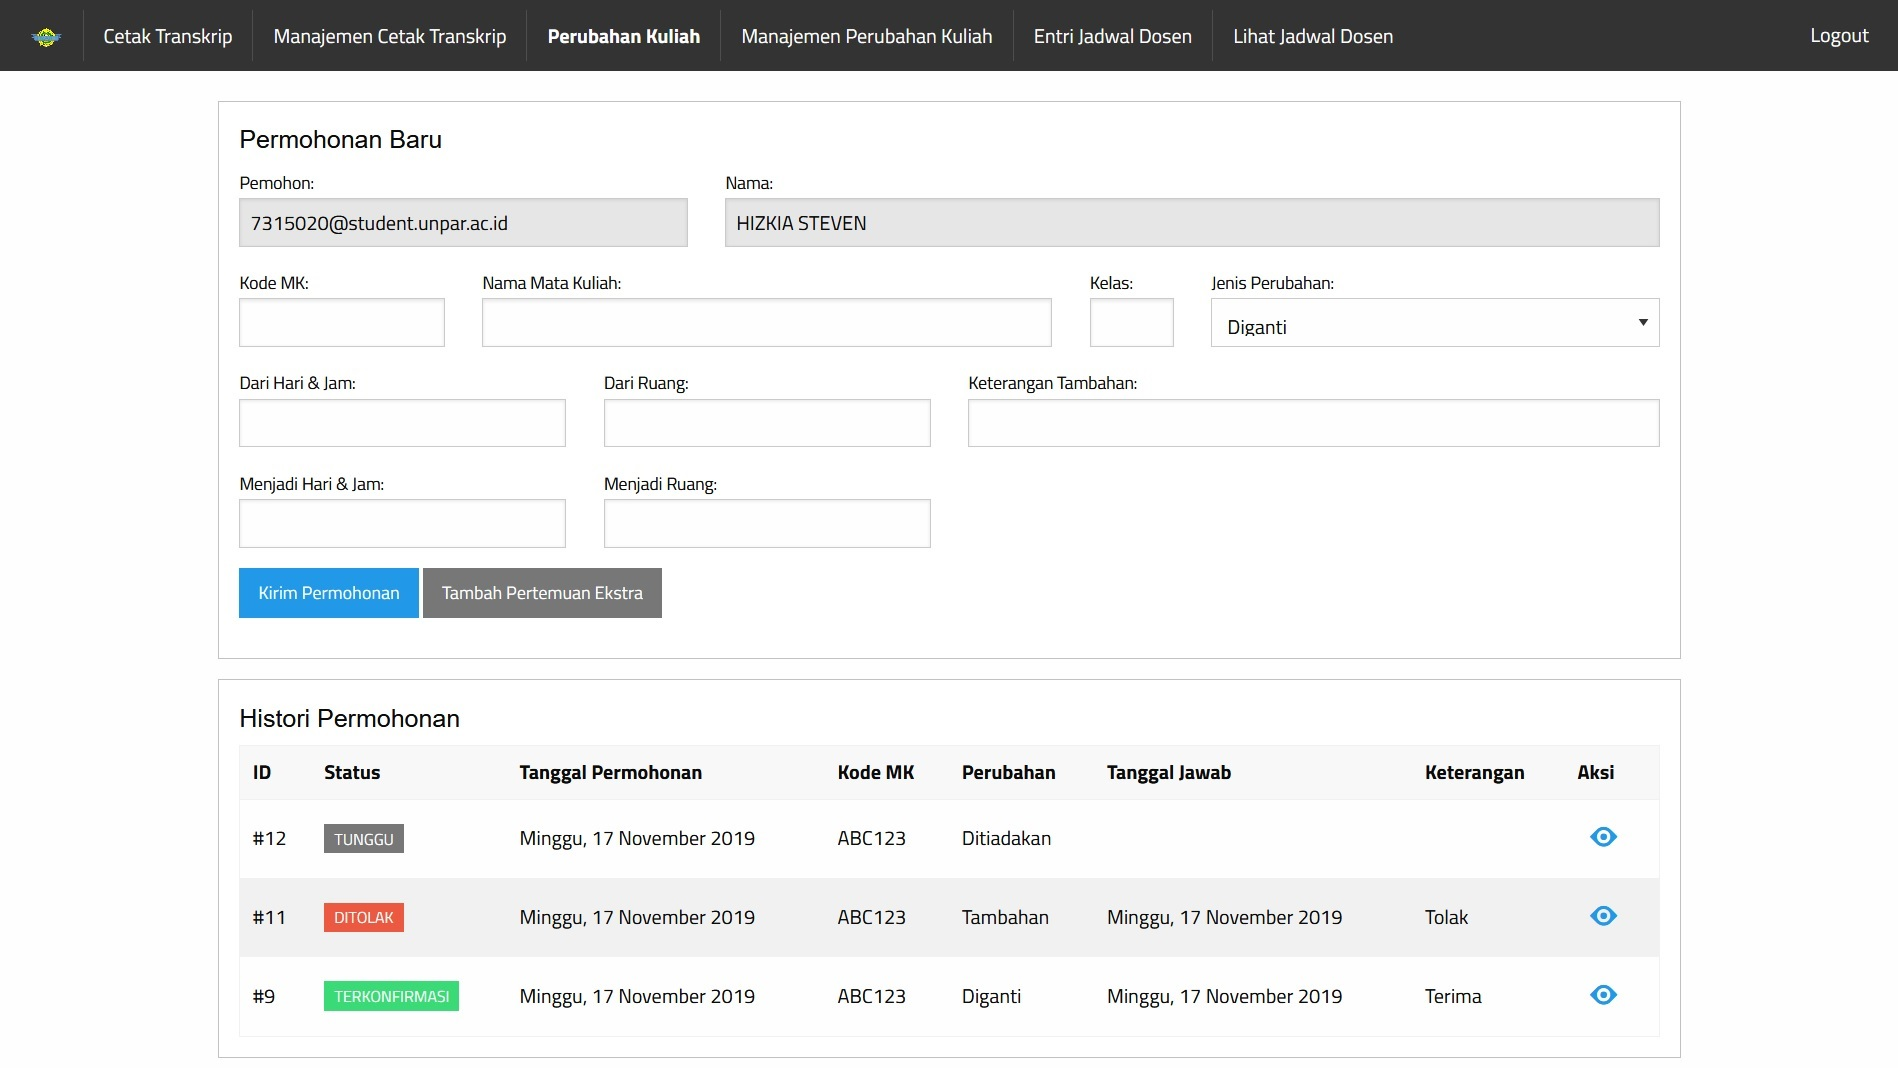
\includegraphics[scale=0.4, frame]{bluetape_perubahan_kuliah}
    \caption[Halaman Perubahan Kuliah Web BlueTape]{Halaman Perubahan Kuliah Web BlueTape}
    \label{fig:bluetape_perubahan_kuliah}
\end{figure}

\subsection{Pengguna Merupakan Dosen Informatika}
\label{sec:bluetape_dosen_informatika}

\subsubsection{Entri Jadwal Dosen}
\label{sec:bluetape_entri_jadwal_dosen}
Pengguna dapat menggunakan menu ini untuk mengisi jadwal mingguan miliknya. Hasilnya dapat diekspor ke dalam dokumen XLS, atau dapat dilihat oleh mahasiswa Informatika melalui portal BlueTape. Tampilan halaman entri jadwal dosen pada web BlueTape dapat dilihat pada \mbox{Gambar \ref{fig:bluetape_entri_jadwal_dosen}}.

\begin{figure}[h]
    \centering  
    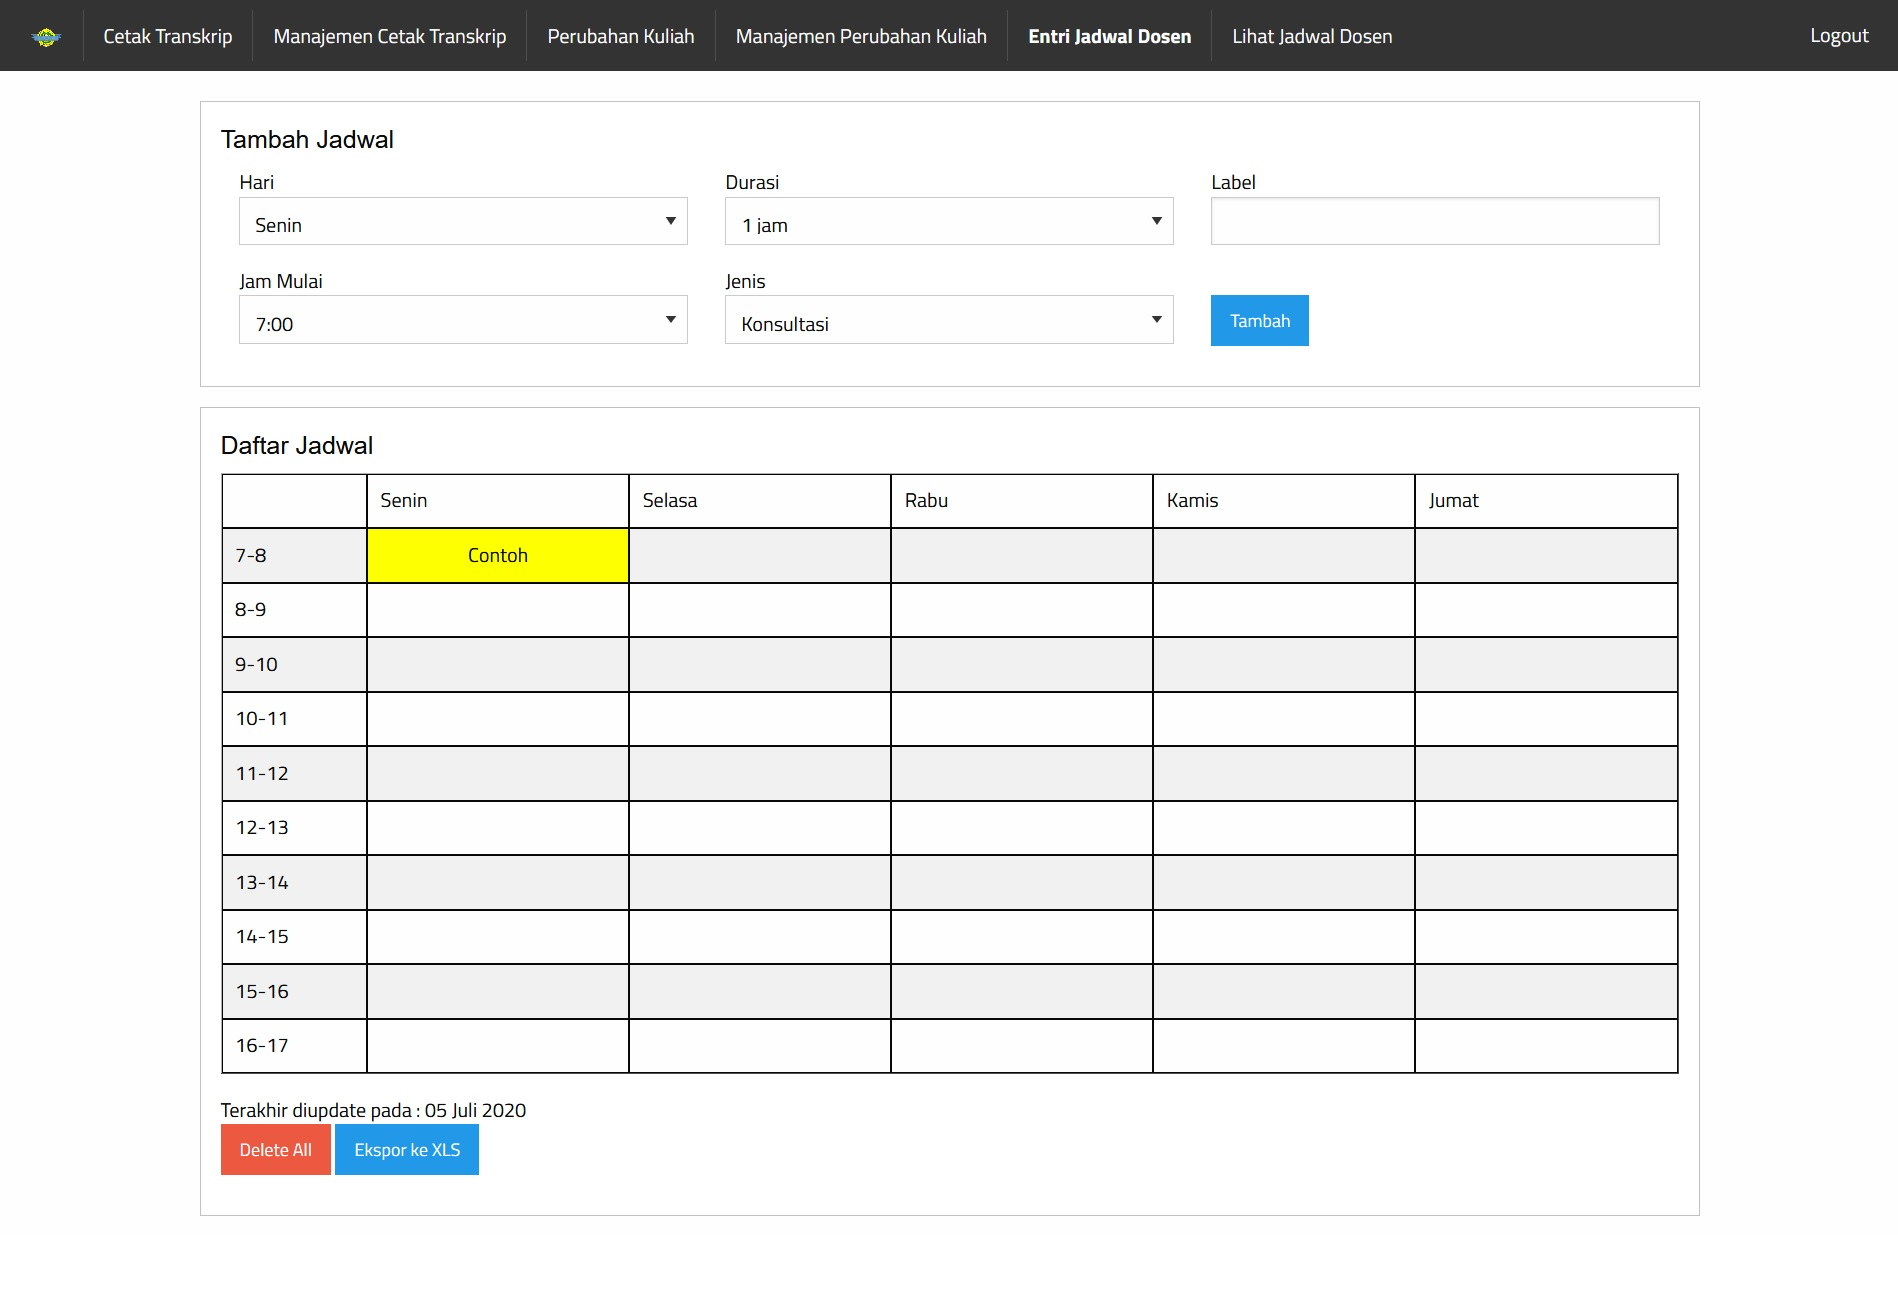
\includegraphics[scale=0.4, frame]{bluetape_entri_jadwal_dosen}
    \caption[Halaman Entri Jadwal Dosen Web BlueTape]{Halaman Entri Jadwal Dosen Web BlueTape}
    \label{fig:bluetape_entri_jadwal_dosen}
\end{figure}

\paragraph{Tambah Jadwal}
\label{sec:bluetape_tambah_jadwal}
\phantom{blank}\\

Bagian paling atas adalah formulir untuk menambahkan entri jadwal, pada bagian tersebut pengguna bisa mengisikan hari, jam mulai, durasi, label, dan jenisnya. Berikut adalah penjelasan jenis yang dapat dipilih:
\begin{itemize}
	\item Konsultasi: Waktu yang pengguna siapkan untuk konsultasi mahasiswa. Pada tabel, bagian ini akan diberi latar belakang warna kuning.
	\item Terjadwal: Kegiatan mingguan lain milik pengguna yang telah terjadwal, contohnya rapat jurusan.
	\item Kelas: Kelas kuliah maupun praktikum.
\end{itemize}

Pengguna dapat menambahkan entri baru dengan menekan tombol "Tambah".

\paragraph{Ubah/Hapus Jadwal}
\label{sec:bluetape_ubah_hapus_jadwal}
\phantom{blank}\\

Pengguna dapat menekan jadwal yang tertera pada tabel untuk mengubahnya. \textit{Pop-up window} akan terbuka dengan pilihan-pilihan yang sama seperti saat menambah jadwal baru. Pada \textit{pop-up} yang sama, pengguna juga bisa menekan tombol "Hapus" untuk menghapus jadwal tersebut.

\paragraph{Hapus Semua}
\label{sec:bluetape_hapus_semua}
\phantom{blank}\\

Pengguna dapat menekan tombol "\textit{Delete All}" untuk secara cepat menghapus seluruh jadwal yang telah dibuat. Bagian ini umumnya digunakan pada awal semester, ketika jadwal pengguna benar-benar baru.

\paragraph{Ekspor ke XLS}
\label{sec:bluetape_ekspor_ke_xls}
\phantom{blank}\\

Pengguna dapat menekan tombol "Ekspor ke XLS" untuk membuat dokumen XLS untuk jadwal miliknya.\footnote{Pada saat skripsi ini dibuat, terdapat \textit{bug} yang menyebabkan dokumen hasil ekspor korup}

\subsection{Pengguna Merupakan Mahasiswa}
\label{sec:bluetape_mahasiswa}

\subsubsection{Cetak Transkrip}
\label{sec:bluetape_cetak_transkrip}
Pengguna dapat menggunakan menu ini untuk mengirimkan permohonan cetak transkrip.

Untuk mengirimkan permohonan pencetakan transkrip, pengguna dapat mengisikan kolom-kolom pada formulir "Permohonan Baru". Pengguna harus mengisi kolom "Keperluan" karena bagian tersebut akan menentukan apakah permohonan pengguna disetujui oleh Tata Usaha atau tidak.

Pengguna hanya dapat mengirimkan permohonan:
\begin{itemize}
	\item Maksimal satu kali dalam satu semester (kecuali jika permohonan ditolak).
	\item Jika masih ada permohonan yang belum dijawab.
\end{itemize}

Umumnya, Tata Usaha akan mencetakkan transkrip mahasiswa dalam waktu satu hari kerja. Jika pengguna mengalami kesulitan, pengguna dapat menghubungi petugas Tata Usaha. Setelah permohonan pengguna disetujui dan dicetak (atau ditolak), pengguna akan mendapatkan notifikasi melalui surel. Tampilan halaman cetak transkrip pada web BlueTape dapat dilihat pada \mbox{Gambar \ref{fig:bluetape_cetak_transkrip}}.

\begin{figure}[H]
    \centering  
    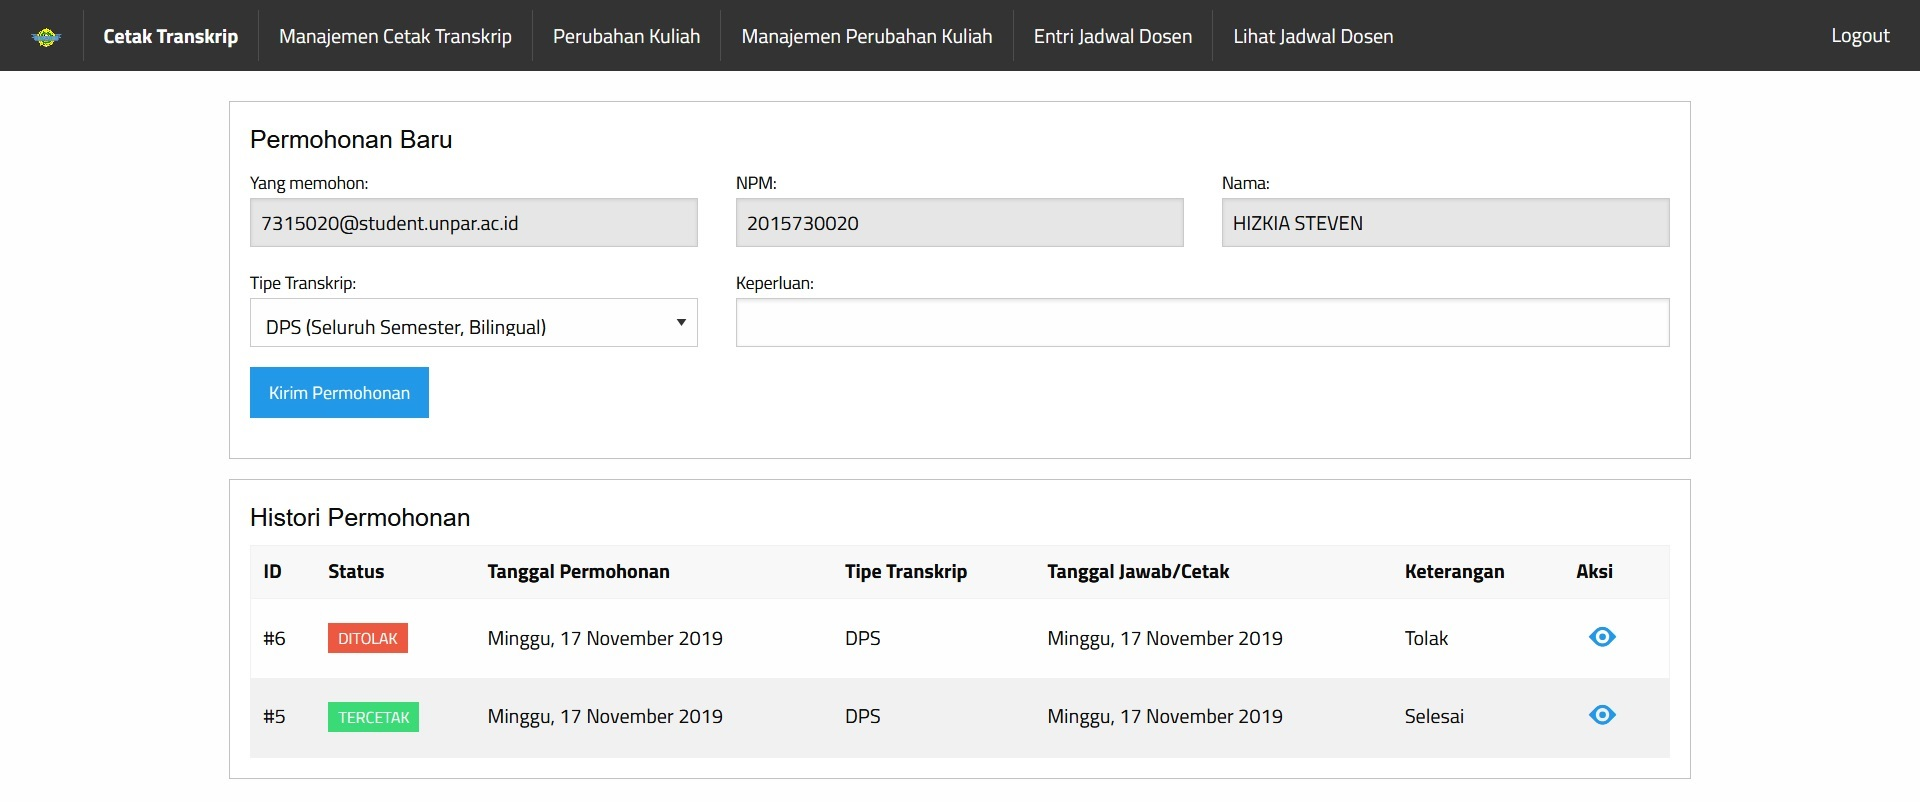
\includegraphics[scale=0.4, frame]{bluetape_cetak_transkrip}
    \caption[Halaman Cetak Transkrip Web BlueTape]{Halaman Cetak Transkrip Web BlueTape}
    \label{fig:bluetape_cetak_transkrip}
\end{figure}

\subsection{Pengguna Merupakan Mahasiswa Informatika}
\label{sec:bluetape_mahasiswa_informatika}

\subsubsection{Lihat Jadwal Dosen}
\label{sec:bluetape_lihat_jadwal_dosen}

Modul ini digunakan untuk melihat jadwal mingguan seluruh dosen Informatika yang telah mendaftarkan jadwalnya.

Pengguna dapat melihat jadwal dosen dengan memilih dosen yang bersangkutan pada seleksi \textit{tab} di bagian atas, jadwal dosen yang bersangkutan akan ditampilkan pada tabel di bagian bawah. Di bawah tabel tersebut, terdapat informasi mengenai waktu terakhir jadwal tersebut diperbarui oleh dosen yang bersangkutan. Informasi ini dapat membantu untuk menentukan, apakah jadwal yang terlihat merupakan jadwal semester lalu, atau sudah diperbarui pada semester ini.

Pengguna dapat menekan tombol "Ekspor ke XLS" untuk mendapatkan jadwal tersebut dalam format XLS, yang kemudian dapat disimpan atau dicetak. Tampilan halaman lihat jadwal dosen pada web BlueTape dapat dilihat pada \mbox{Gambar \ref{fig:bluetape_lihat_jadwal_dosen}}.

\begin{figure}[H]
    \centering  
    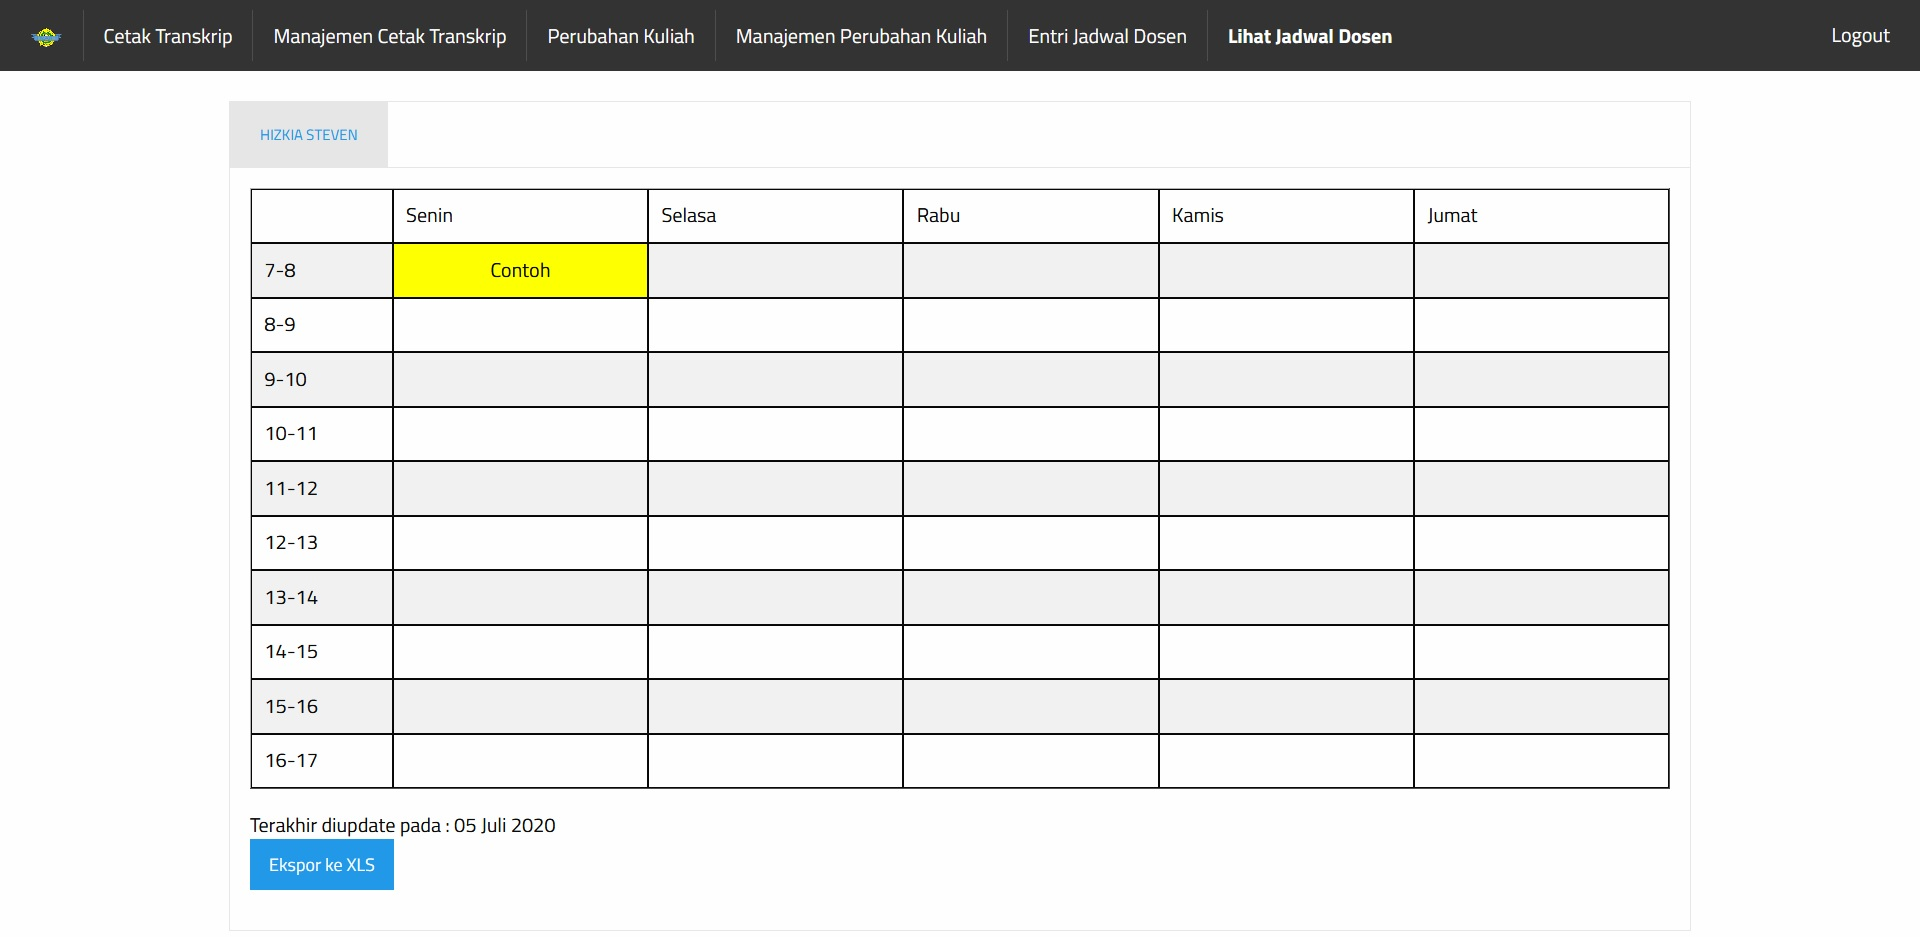
\includegraphics[scale=0.4, frame]{bluetape_lihat_jadwal_dosen}
    \caption[Halaman Lihat Jadwal Dosen Web BlueTape]{Halaman Lihat Jadwal Dosen Web BlueTape}
    \label{fig:bluetape_lihat_jadwal_dosen}
\end{figure}

\subsection{Pengguna Merupakan Staf Tata Usaha}
\label{sec:bluetape_staf_tata_usaha}

\subsubsection{Manajemen Perubahan Kuliah}
\label{sec:bluetape_manajemen_perubahan_kuliah}
Modul ini berguna untuk melakukan manajemen permintaan perubahan kuliah. Saat pengguna memasuki modul ini, tabel akan menampilkan daftar permohonan, terurut tanggal.

Ada beberapa tombol yang tersedia untuk setiap permohonan:
\begin{itemize}
	\item Tombol dengan ikon mata, untuk melihat detail permohonan, berguna untuk memahami permohonan lebih lanjut dan menentukan apakah permohonan disetujui atau tidak.
	\item Tombol dengan ikon mesin cetak, untuk membuka \textit{pop-up} untuk mencetak \textit{print-out} pengumuman. Pengguna cukup mencetak sebanyak yang dibutuhkan, serta mengedarkan ke staf/pekarya terkait.
	\item Tombol dengan ikon ibu jari mengarah ke atas, untuk mengonfirmasi bahwa pengumuman sudah dicetak dan disebarkan.
	\item Tombol dengan ikon ibu jari mengarah ke bawah, untuk menyatakan bahwa permohonan ini ditolak. Jika permohonan ditolak, maka pengguna harus mengisi bagian alasan agar tidak membingungkan pemohon.
	\item Tombol dengan ikon keranjang, untuk menghapus permohonan secara permanen. Pengguna disarankan untuk tidak pernah menggunakan tombol ini kecuali jika terpaksa.
\end{itemize}

Tampilan halaman manajemen perubahan kuliah pada web BlueTape dapat dilihat pada \mbox{Gambar \ref{fig:bluetape_manajemen_perubahan_kuliah}}.

\begin{figure}[H]
    \centering  
    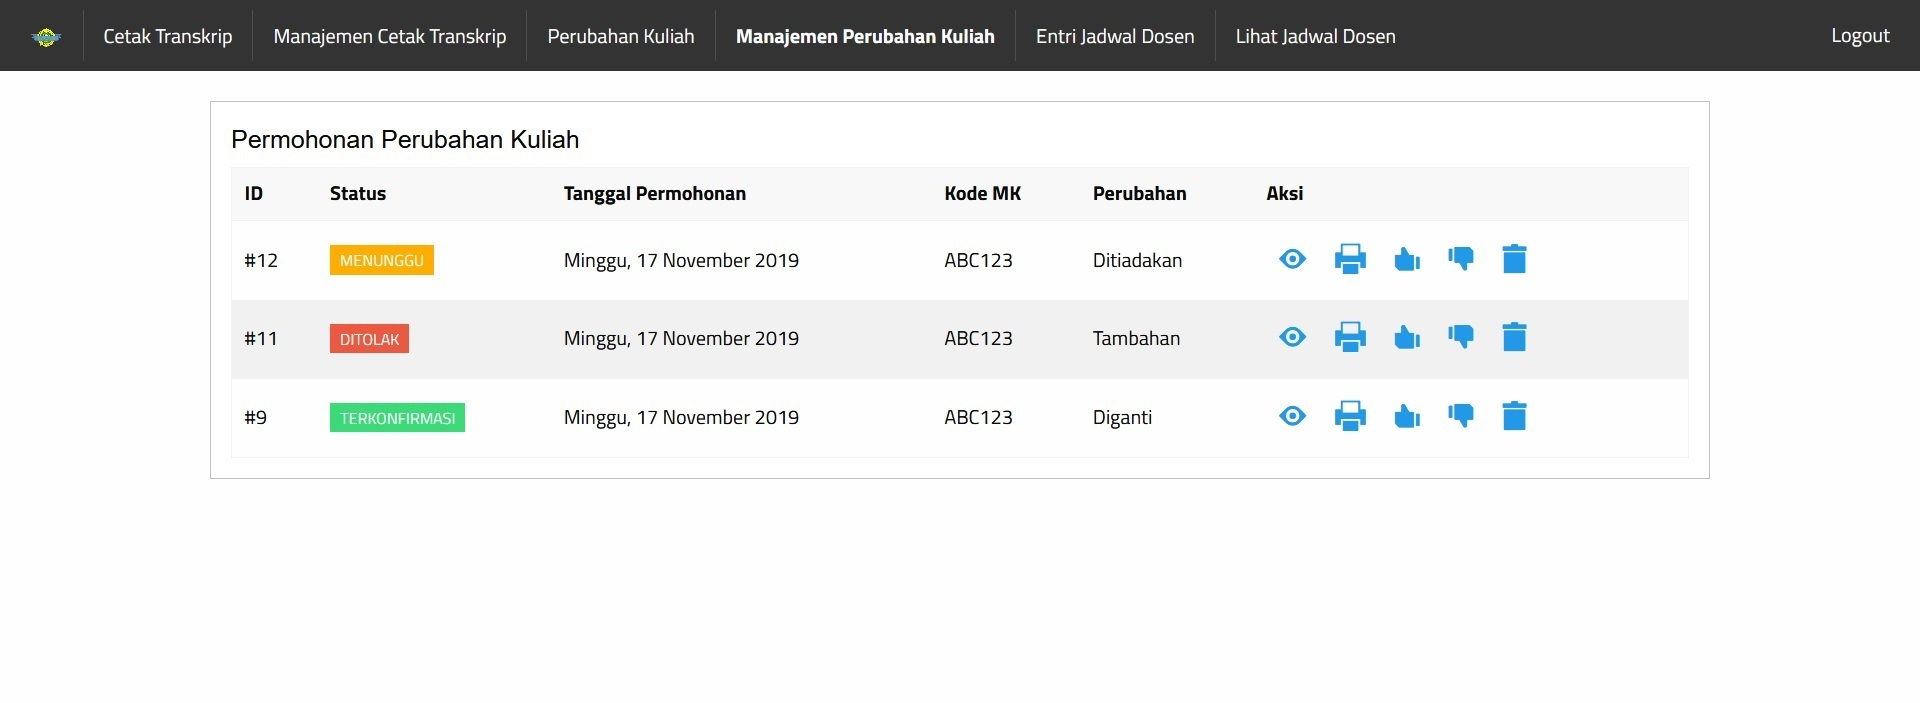
\includegraphics[scale=0.4, frame]{bluetape_manajemen_perubahan_kuliah}
    \caption[Halaman Manajemen Perubahan Kuliah Web BlueTape]{Halaman Manajemen Perubahan Kuliah Web BlueTape}
    \label{fig:bluetape_manajemen_perubahan_kuliah}
\end{figure}

\subsubsection{Manajemen Cetak Transkrip}
\label{sec:bluetape_manajemen_cetak_transkrip}
Daftar permintaan transkrip disajikan dalam bentuk tabel. Hanya informasi penting saja yang ditampilkan, sedangkan untuk melihat detil yang lebih lengkap pengguna dapat menekan tombol dengan ikon mata (detail). Terdapat dua pilihan jawaban yaitu tolak (tombol dengan ikon ibu jari mengarah ke bawah) dan cetak (tombol dengan ikon mesin cetak). Masing-masing memerlukan keterangan tambahan (alasan ditolak atau komentar cetak). Jika memungkinkan, BlueTape akan menampilkan tautan ke halaman DPS (Daftar Perkembangan Studi) mahasiswa yang bersangkutan di dialog cetak.

Modul ini berguna untuk melakukan manajemen permohonan pencetakan transkrip. Saat pengguna memasuki modul ini, tabel akan menampilkan daftar permohonan, terurut tanggal. Pengguna juga bisa mencari permintaan berdasarkan NPM (Nomor Pokok Mahasiswa).

Ada beberapa tombol yang tersedia untuk setiap permohonan:
\begin{itemize}
	\item Tombol dengan ikon mata, untuk melihat detail permohonan, berguna untuk memahami permohonan lebih lanjut dan menentukan apakah permohonan disetujui atau tidak.
	\item Tombol dengan ikon ibu jari mengarah ke bawah, untuk menyatakan bahwa permohonan ini ditolak. Jika permohonan ditolak, maka pengguna harus mengisi bagian alasan agar tidak membingungkan pemohon.
	\item Tombol dengan ikon mesin cetak, untuk membuka \textit{pop-up} untuk untuk mengonfirmasi bahwa transkrip telah tercetak. Di \textit{pop-up} ini juga akan tersedia tautan menuju halaman pencetakan transkrip pada SIAKAD.
	\item Tombol dengan ikon keranjang, untuk menghapus permohonan secara permanen. Pengguna disarankan untuk tidak pernah menggunakan tombol ini kecuali jika terpaksa.
\end{itemize} 

Tampilan halaman manajemen cetak transkrip pada web BlueTape dapat dilihat pada \mbox{Gambar \ref{fig:bluetape_manajemen_cetak_transkrip}}.

\begin{figure}[H]
    \centering  
    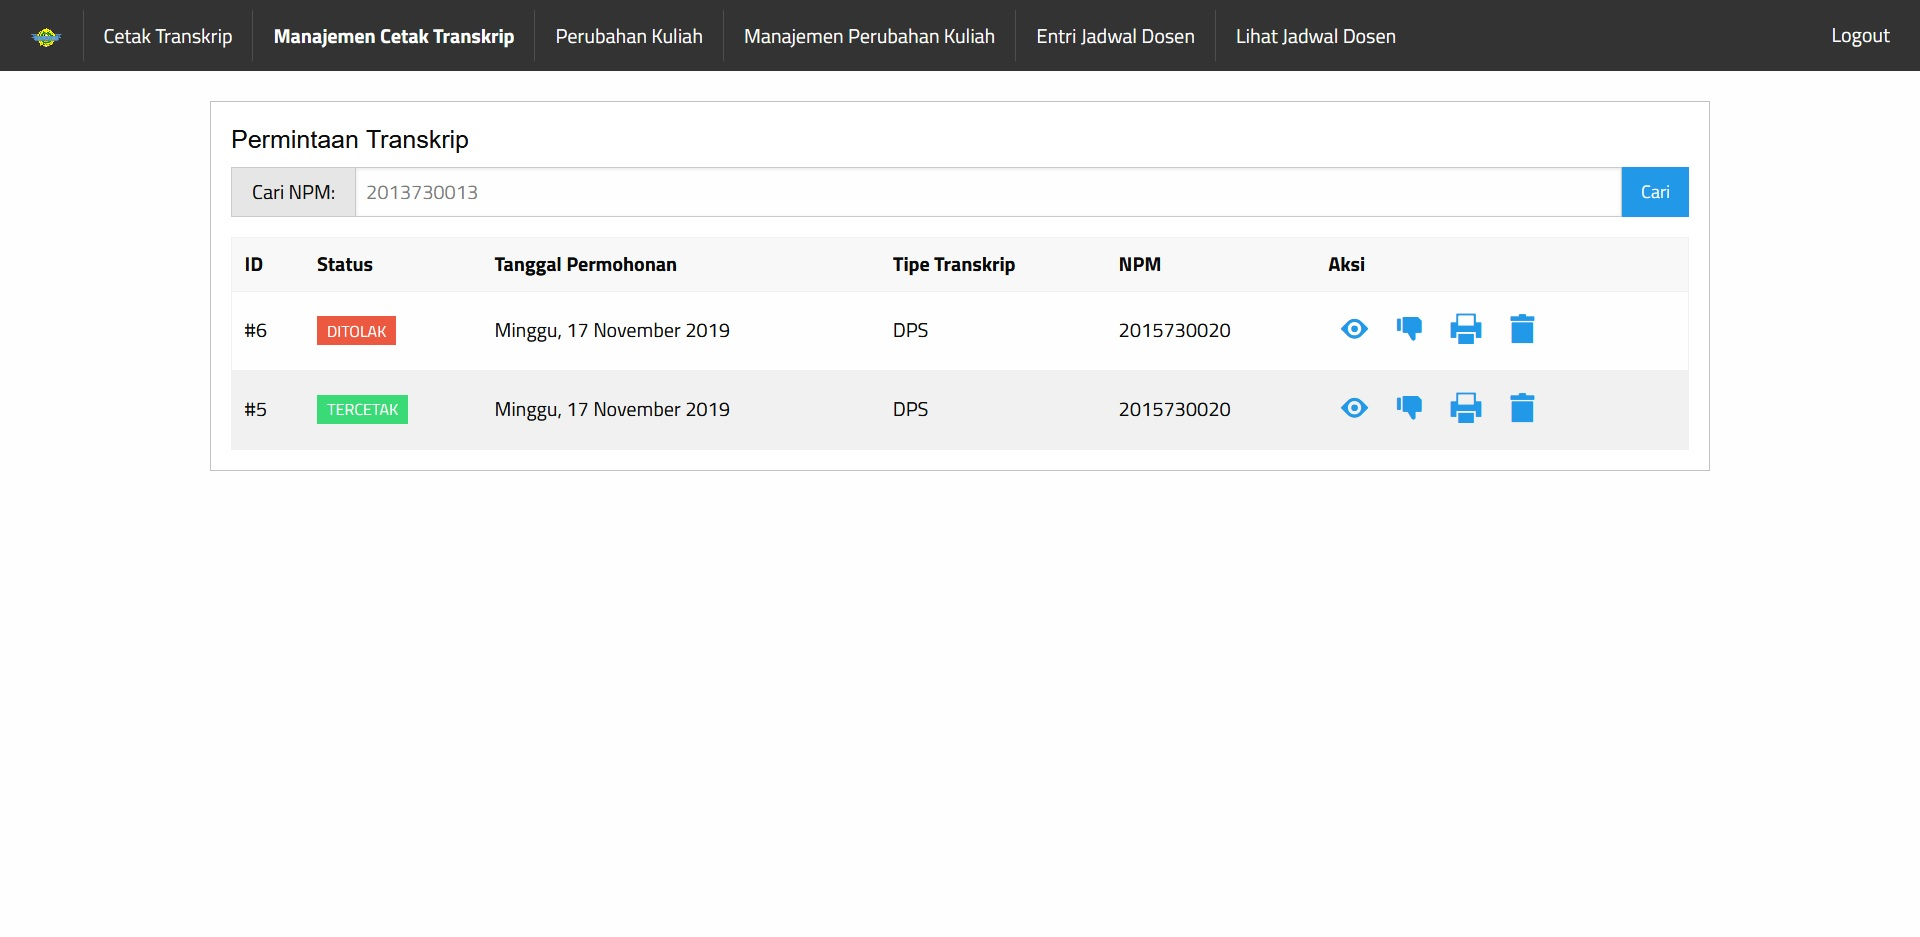
\includegraphics[scale=0.4, frame]{bluetape_manajemen_cetak_transkrip}
    \caption[Halaman Manajemen Cetak Transkrip Web BlueTape]{Halaman Manajemen Cetak Transkrip Web BlueTape}
    \label{fig:bluetape_manajemen_cetak_transkrip}
\end{figure}